\cleardoublepage
\chapter{Tests, Results and Analysis}\label{chap:Tests}
% To do: 
% Color Scheme
% Red - Not started
% Yellow - In progress
% Blue - Done, under approval
% Green - Done and approved
\todo[inline,color=blue!40]{closed - v1.1 finished 16/07/2021, to review}
%\todo[inline,color=red!40]{*Chapter Introduction}
%\todo[inline,color=blue!40]{*1 - Algorithm Test}
%\todo[inline,color=blue!40]{*2 - Microphone Tests}
%\todo[inline,color=blue!40]{*3 - Accelerometer and PiezoElectric Tests}
%\todo[inline,color=blue!40]{*4 - Identification algorithm Tests}
%% Writing %%%%%%%%%%%%%%%%%%%%%%%%%%%%%%%%%%%%%%%%%%%%%%%%%%%%%%%%%%%%
This chapter is dedicated to explore the development of the practical tests, with the purpose to verify if the application of these techniques is valid for a future product. For that the setups, hardware and software were tested. Along the the chapter is explained how each test was performed and what was the purpose of each of them, with the final test being the one to the identification validation. 
\section{Algorithm Test}
The purpose of this, is to test the effectiveness of the algorithm implementation, mentioned in~\ref{subsec:fftImp}, one way to perform this test is recurring to random signals with known frequencies, this way is possible to compare the results from the implementation in a microcontroller environment with the absolute frequency determined when generation the random signal.

To try to perform the tests as close as possible to the type of signals that were expected to obtain, several aspects were taken into consideration, for that reason a small explanation of how the signals were generated will be given. 
%----------------Introduction above this line--------------------------
\subsection{Signal Generation}\label{subsec:sigGen}
To try to synthesis a wave form as similar as possible to the one resulting from the work of~\citeauthor{wuLiquidLevelDetector2014b} in figure~\ref{fig:realsignalWu}.
\begin{figure}[]
    \centering
    \begin{subfigure}{0.45\textwidth}
        \centering
        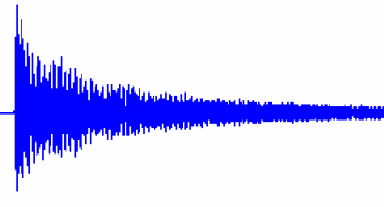
\includegraphics[width=\linewidth]{Chapters/6CHP/Figures/completesignalWu.pdf}
        \caption{Complete Signal}{}
        %\label{subfig:g1lines}
    \end{subfigure}
    \begin{subfigure}{0.45\textwidth}
        \centering
        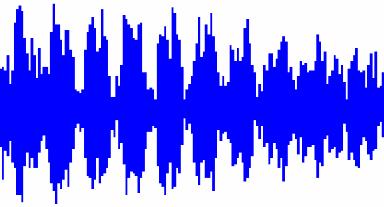
\includegraphics[width=\linewidth]{Chapters/6CHP/Figures/fractionWu.pdf}
        \caption{Fraction of the signal}{}
        %\label{subfig:g2lines}
    \end{subfigure}
    \caption{Real signal}{~\cite{wuLiquidLevelDetector2014b}}
     \label{fig:realsignalWu}
 \end{figure}
First is randomly define a frequency to be the dominant and a regular wave was generated, to create the decay effect the resulting wave is multiplied by $\frac{1}{e^{x}}$ being $x=1$, creating the echo effect by adding the original wave multiplied by the same equation, increasing the value of $x$ and adding the wave to the original shifting N/16, with N being the original size of the wave. This procedure is repeated to generate more waves with different frequencies and smaller amplitudes, in the end random noise is added with random variance, being at maximum half of the signal generated without any noise. An example of the resulting waves can be observed in the figure~\ref{fig:synthetizedSignal}.
\begin{figure}[]
    \centering
    \begin{subfigure}{0.45\textwidth}
        \centering
        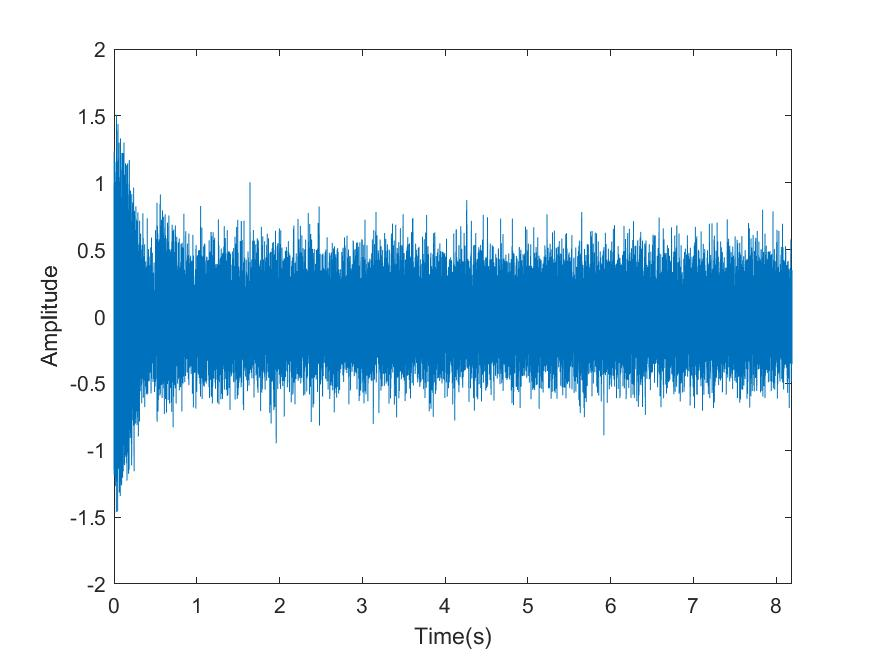
\includegraphics[width=\linewidth]{Chapters/6CHP/Figures/signal1.jpg}
        \caption{Noise variance of 0.05}{}
        %\label{subfig:g1lines}
    \end{subfigure}
    \begin{subfigure}{0.45\textwidth}
        \centering
        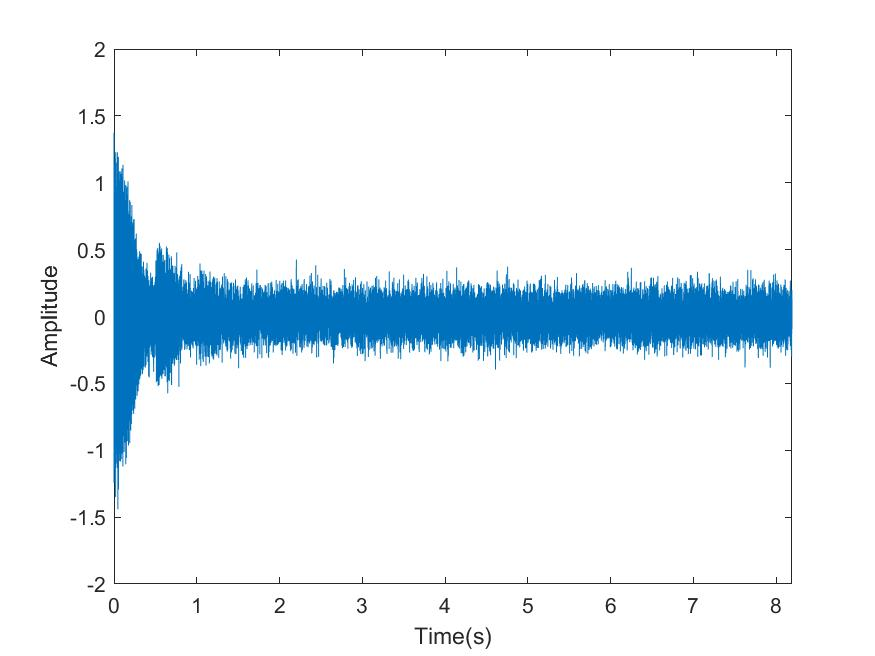
\includegraphics[width=\linewidth]{Chapters/6CHP/Figures/signal2.jpg}
        \caption{Noise variance of 0.01}{}
        %\label{subfig:g2lines}
    \end{subfigure}
    \begin{subfigure}{0.45\textwidth}
        \centering
        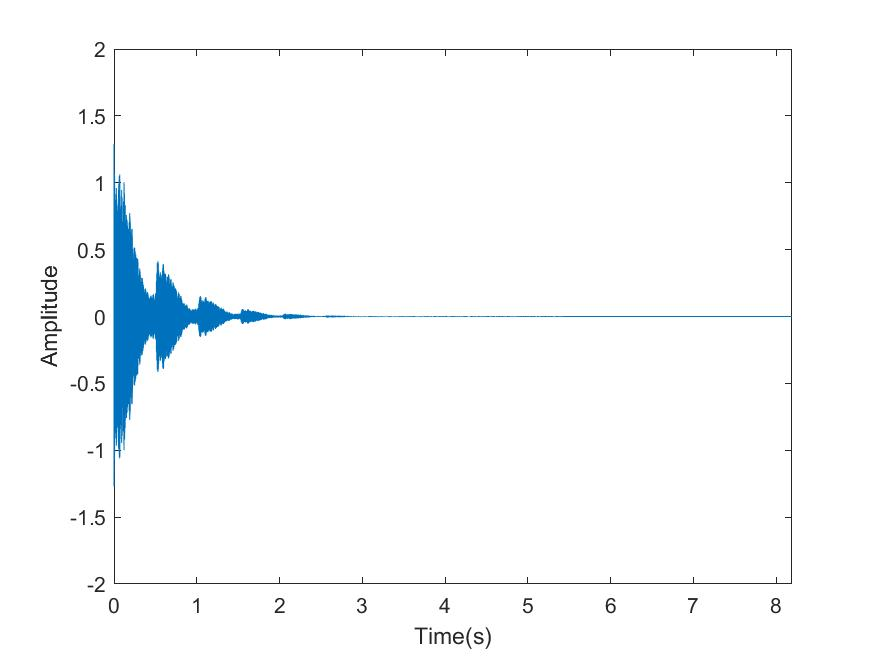
\includegraphics[width=\linewidth]{Chapters/6CHP/Figures/signal3.jpg}
        \caption{Noise variance of 0}{}
        %\label{subfig:g1lines}
    \end{subfigure}
    \begin{subfigure}{0.45\textwidth}
        \centering
        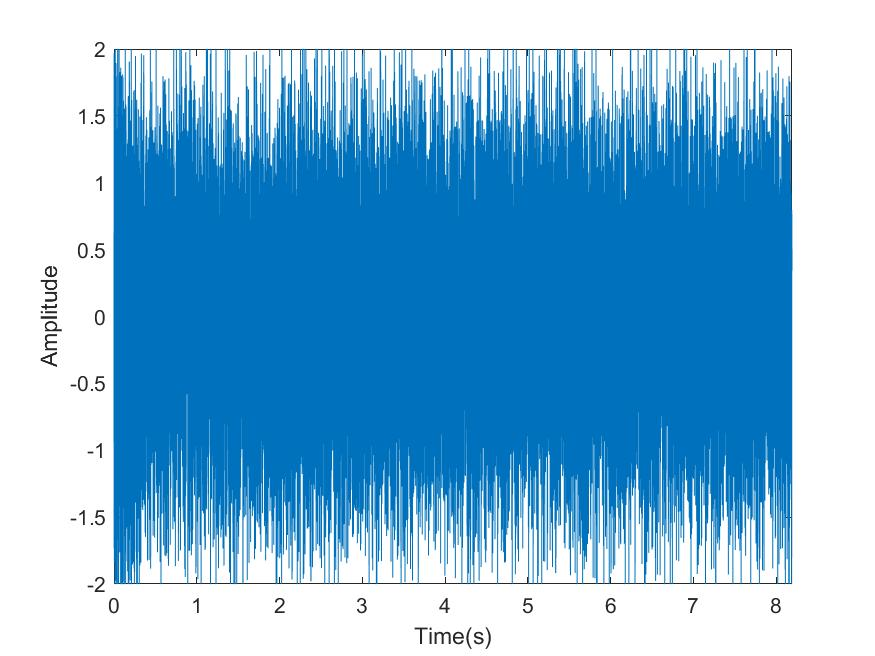
\includegraphics[width=\linewidth]{Chapters/6CHP/Figures/signal4.jpg}
        \caption{Noise variance of 0.5}{}
        %\label{subfig:g2lines}
    \end{subfigure}
    \caption{Example of signals synthetized with \acrshort{matlab} with different noise variances}{}
     \label{fig:synthetizedSignal}
 \end{figure}
\subsection{Tests}
To test the effectiveness of the \acrshort{fft} algorithm in use, where performed in total 1000 tests to verify the obtained error of the implementation. The tests weren't only performed to the Fixed-Point algorithm in the microcontroller, the same code used in the microcontroller was also implemented in a \acrshort{pc} and the \acrshort{fft} function of \acrshort{matlab} was used as a control test, to verify that the signal wasn't to corrupted with noise that even \acrshort{matlab} wasn't able to determine the dominant frequency correctly.

In a \acrshort{pc} environment was implemented both \acrshort{fft}s, the Fixed-Point and the Floating-Point, in the microcontroller it was only possible to perform tests with the Fixed-Point since the other version exceeded the amount of memory needed to use the implementation. In each test a random signal was generated, as mentioned in~\ref{subsec:sigGen}, 512 samples of that signal were selected and converted to values between 0 and 1023, just like if it was converted by an \acrshort{adc}. After generating the signal, the dominant frequency is saved, to compare with the results, the samples are processed in \acrshort{matlab} and a dominant frequency is obtained and saved as well. The samples used in \acrshort{matlab} environment are saved, in order to be tested in both implementations in the \acrshort{pc} environment and the obtained results are saved. To finalize the samples are sent to the microcontroller and processed and the result is sent back to the \acrshort{pc} and saved. After all the tests, the results obtained are compared with the original value used in the frequency, allowing to verify how the algorithm performs. 
\begin{figure}[]
    \centering
    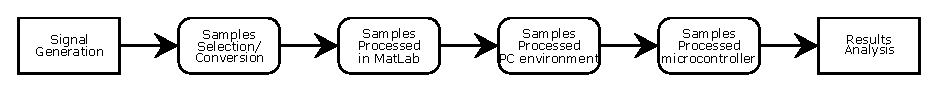
\includegraphics[width=1\textwidth]{Chapters/6CHP/Figures/ProcFlow.eps}
    \caption{Flow of signal processing in different environments}{}
    \label{fig:flowProc}
\end{figure}
Although the tests were performed in other environments, the test that is the most important is the one in the microcontroller. In the tests performed in the microcontroller not only the validity of the implementation, but it is also necessary to know how long it takes to execute the algorithm in the microcontroller and what are the memory needs of the program. The program that executes the algorithm was built to start measuring the execution time of the \acrshort{fft} implementation right before it starts, and end it after calculated the magnitude of the resulting signal, to measure how long takes to perform these tasks it uses one of the timers that the microcontroller has. To better understand how all works, observe figure\ref{fig:dataProcuC}.
\begin{figure}[]
    \centering
    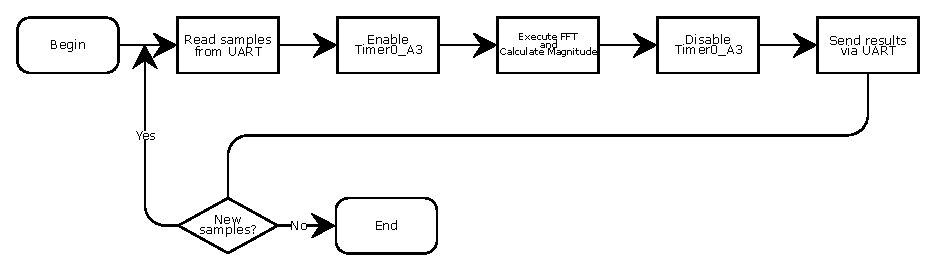
\includegraphics[width=1\textwidth]{Chapters/6CHP/Figures/uCDataProc.eps}
    \caption{Flow of processing in the microcontroller}{}
    \label{fig:dataProcuC}
\end{figure}
\subsection{Results}
The resulting data obtained is the dominant frequency of each implementation with the \acrshort{fft}, additionally in the microcontroller option was also measured the execution time of the algorithm. In the resulting dominant frequency from all cases was then compared with the absolute frequency that was saved every time that a new signal was generated, the error obtained in each implementation can be observed in the table~\ref{tab:perfRes}.
\begin{table}
    \centering
    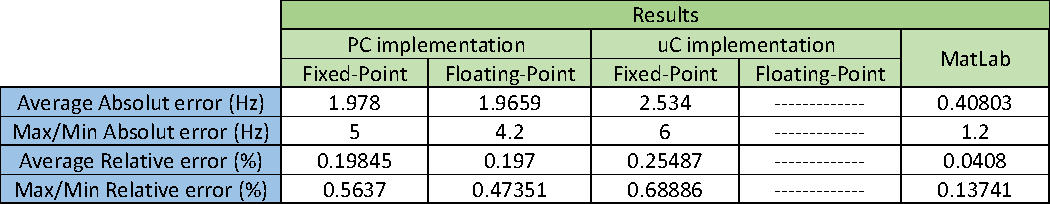
\includegraphics[width=1\textwidth]{Chapters/6CHP/Figures/performanceAlgorithm.pdf}
    \caption{Results of the execution of a synthetic signal in the different algorithms}
    \label{tab:perfRes}
\end{table}
Is evident that the results from \acrshort{matlab} are much better when compared with the rest and when comparing the Floating-Point with the Fixed-Point, in the \acrshort{pc} results, there is a slight difference between the two, but for the microcontroller in use wasn't possible to implement the Floating-Point, anyway the error obtained in the Fixed-Point doesn't increase significatively, with these results the use of the implementation is expected to be precise for the application. 

The results of the execution time of the algorithm can be observed in table~\ref{tab:excTimeuC}, the number of ticks is due the fact that to measure the execution time, a timer was configured to generate an interruption every 500$\mu$s, incrementing a variable each time that happen, as a result, by multiplying the number of ticks by the time each interruption is generated, gives the execution time of the algorithm. Taking into consideration that microcontroller has a small processing power and the embedded Hardware Multiplier hasn't been used, around 3s to process 512 samples it is to long, but acceptable under the test circumstances, since isn't mandatory for the results to be returned in real-time.  
\begin{table}
    \centering
    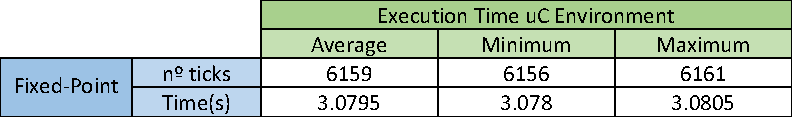
\includegraphics[width=1\textwidth]{Chapters/6CHP/Figures/excTimeuC.pdf}
    \caption{Results of the execution of the Fixed-Point implementation in the microcontroller}
    \label{tab:excTimeuC}
\end{table}
%% Missing memory analysis, do that latter, se in code composer studio the indirect calls of the project
\section{Microphone Test}\label{sec:MicroTests}
\subsection{Signal Capturing and Tests}

There are a few things that should be conclude from the tests with a microphone before starting the analysis with different sensors, they are in the first place the viability of the frequency analysis, for different liquid levels, if valid which is the frequency interval that should be taken into consideration and finally which are the more practical and were the best results are obtained, for latter help selecting the optimal point to place the sensor. 

Considering this, four points were considered to make some measurements, identified in the illustration in figure~\ref{fig:measPointMic}, the points are all in the lateral surface of the \acrshort{lpg} bottle. The bottle in use is divided in two similar parts, by a welding joint in the middle, the lower and the top section, and the measuring points will be the bottom and the middle of each one of the sections, in other words, the points are right above the curvature and in the middle in the lower section and right above the welding joint and the middle of the top section. In some background studies made in chapter~\ref{chap:stArt}, another possibility was under the \acrshort{lpg} bottle but this option isn't practical, to place the microphone nor to hit the LPG bottle.
\begin{figure}[]
    \centering
    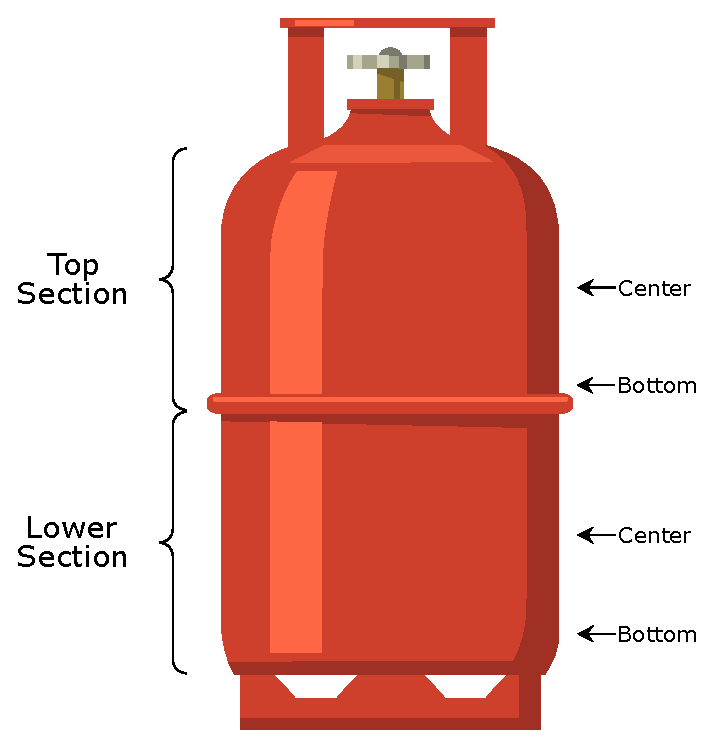
\includegraphics[width=0.35\textwidth]{Chapters/6CHP/Figures/measuringPointsMic.eps}
    \caption{Measuring points in the LPG bottle}{}
    \label{fig:measPointMic}
\end{figure}
In each of the points illustrated was recorded the sound produced when manually hitting the lateral surface of the \acrshort{lpg} bottle, for the 3 bottles available. Each of the 3 bottles contained a different level of liquid, for safety reasons the liquid was water, and they were full, half-full and empty. 

To capture, record and save the sound, some of the \acrshort{matlab} capabilities were used to that purpose, the signal from the microphone was captured with a sampling frequency of 4k$Hz$, according to the table~\ref{tab:sampRat}, to ensure that there was enough time between setting the \acrshort{pc} to record and the manual hit, each saved sample is around 4 seconds, after it the signal can be processed and the resulting data analyzed.
%add here a flux gram
\subsection{Results}
%add images of the signals in the time domain
Several repetitions of the measurements were performed, to guarantee that the results obtained follow a determined pattern and won't vary much from one measurement to another. In the figure~\ref{fig:TimeRealDataMic} are presented the results from the different points of measurement in the different \acrshort{lpg} bottles and in figure~\ref{fig:ProcRealDataMic} the result from processing the same signals. Although is only presented one per point and bottle the remaining results were similar to the ones presented, the main difference for the remaining results can depend on how the hammer hits the surface of the LPG bottle and thus the signal can have smaller/bigger amplitude in the signals in the time domain, or peaks with higher/lower magnitude in the frequency domain.

%Time domain signals
\begin{figure}[]
    \centering
    \begin{subfigure}{0.45\textwidth}
        \centering
        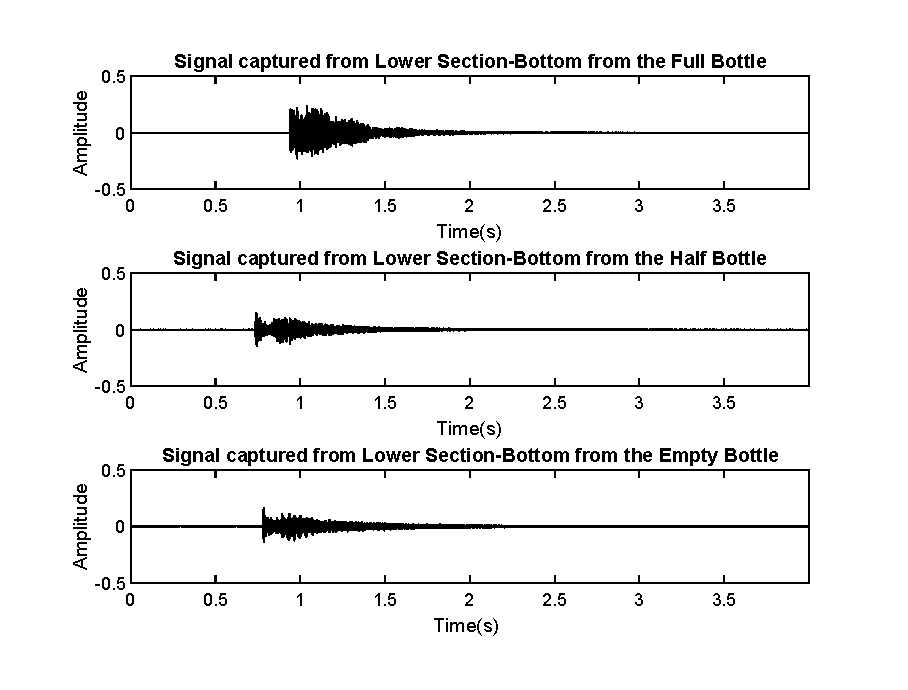
\includegraphics[width=\linewidth]{Chapters/6CHP/Figures/TimeLowBottom.eps}
        \caption{Lower Section, Bottom Position}{}
        \label{subfig:timeLowBotMic}
    \end{subfigure}
    \begin{subfigure}{0.45\textwidth}
        \centering
        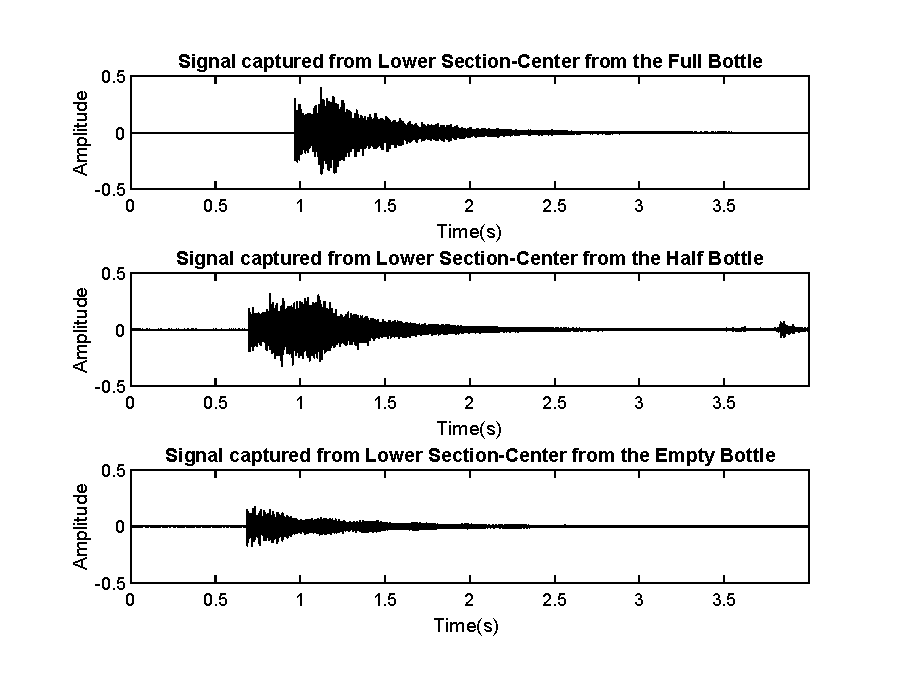
\includegraphics[width=\linewidth]{Chapters/6CHP/Figures/TimeLowCenter.eps}
        \caption{Lower Section, Center Position}{}
        \label{subfig:timeLowCenMic}
    \end{subfigure}
    \begin{subfigure}{0.45\textwidth}
        \centering
        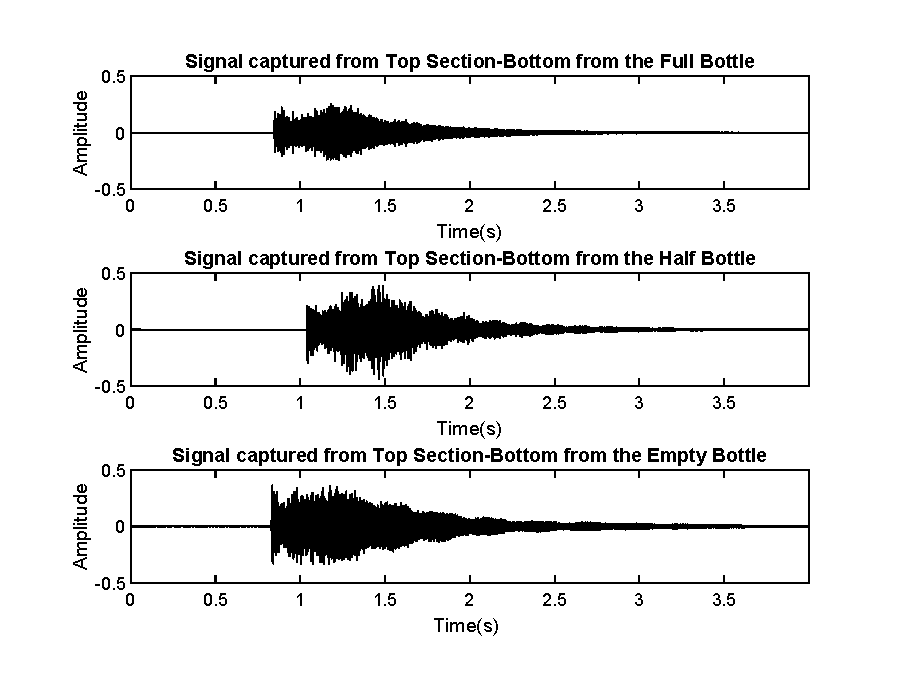
\includegraphics[width=\linewidth]{Chapters/6CHP/Figures/TimeTopBottom.eps}
        \caption{Top Section, Bottom Position}{}
        \label{subfig:timeTopBotMic}
    \end{subfigure}
    \begin{subfigure}{0.45\textwidth}
        \centering
        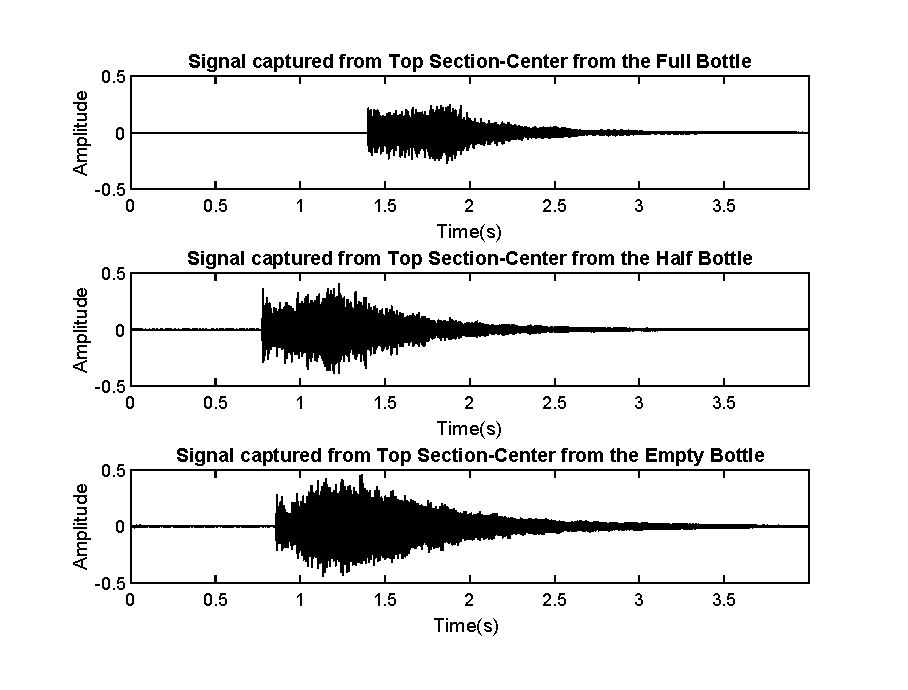
\includegraphics[width=\linewidth]{Chapters/6CHP/Figures/TimeTopCenter.eps}
        \caption{Top Section, Center Position}{}
        \label{subfig:timeTopCenMic}
    \end{subfigure}
    \caption{Captured signals in different locations in the \acrshort{lpg} bottle}{}
     \label{fig:TimeRealDataMic}
\end{figure}

A example of how the hitting of the hammer affects the captured signal can be observed in the figure~\ref{subfig:timeLowCenMic}, where the signal from the empty bottle has a smaller amplitude when compared with the signals captured from the full/half bottle and in the figures~\ref{subfig:timeTopBotMic}\subref{subfig:timeTopCenMic} the same doesn't happen. For this reason, it is also necessary to find alternatives to manual hitting in the \acrshort{lpg} bottle, first because the results won't be constant and second because in a final application it is not practical to do it manually. But for now, the manual hitting was considered.

Even though the time domain isn't considered to the detection of the liquid level, is interesting to observe the results obtained, beside the slight increase of the amplitude in the signal from the full bottle to the empty, the echo also increases in the same way as the amplitude, the the other difference is how long the echo/oscillation occurs, once again from the full bottle to the empty the interval of time that happens increases.

%Latter correct the reference and sub reference above
%Frequency domain signals
\begin{figure}[]
    \centering
    \begin{subfigure}{0.45\textwidth}
        \centering
        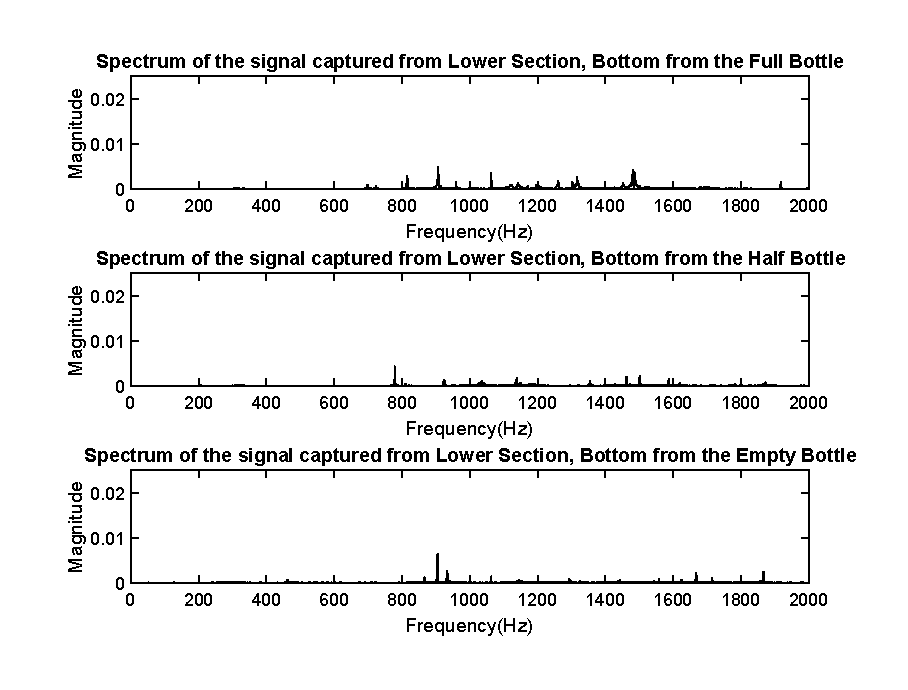
\includegraphics[width=\linewidth]{Chapters/6CHP/Figures/LowBot.eps}
        \caption{Lower Section, Bottom Position}{}
        \label{subfig:LowBotMic}
    \end{subfigure}
    \begin{subfigure}{0.45\textwidth}
        \centering
        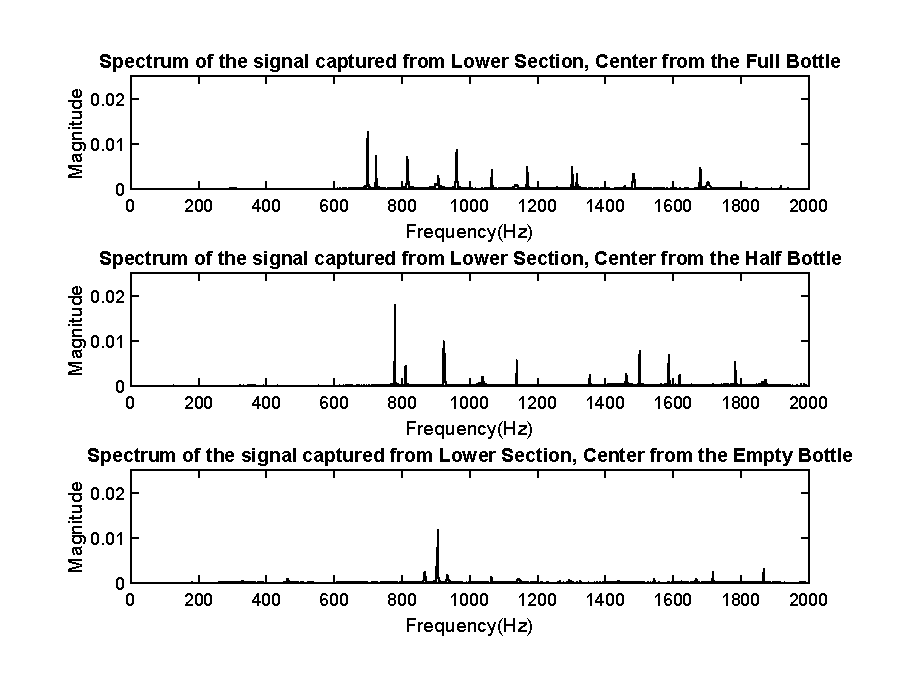
\includegraphics[width=\linewidth]{Chapters/6CHP/Figures/LowCenter.eps}
        \caption{Lower Section, Center Position}{}
        \label{subfig:LowCenMic}
    \end{subfigure}
    \begin{subfigure}{0.45\textwidth}
        \centering
        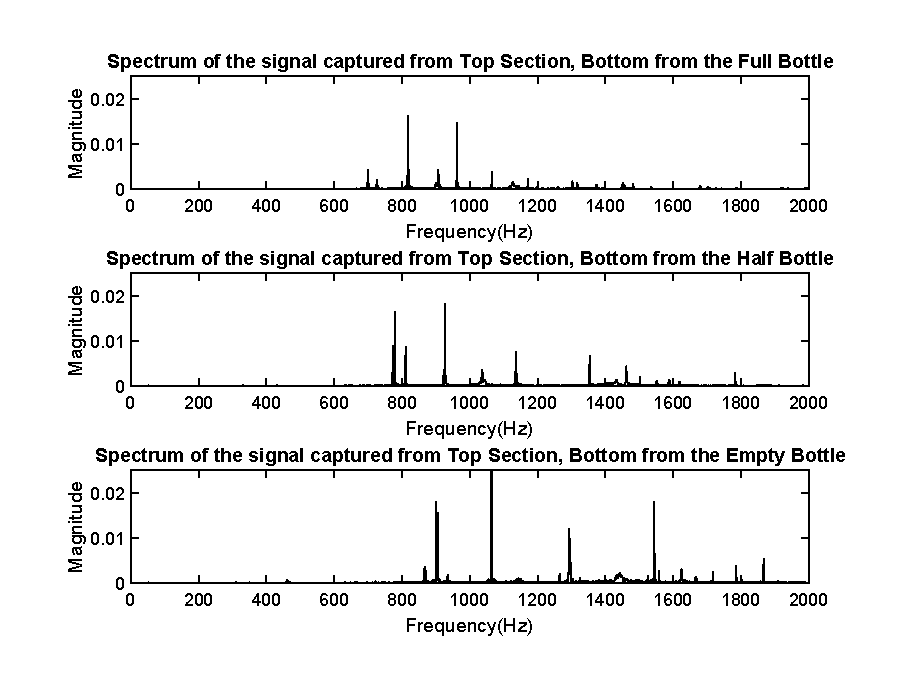
\includegraphics[width=\linewidth]{Chapters/6CHP/Figures/TopBot.eps}
        \caption{Top Section, Bottom Position}{}
        \label{subfig:TopBotMic}
    \end{subfigure}
    \begin{subfigure}{0.45\textwidth}
        \centering
        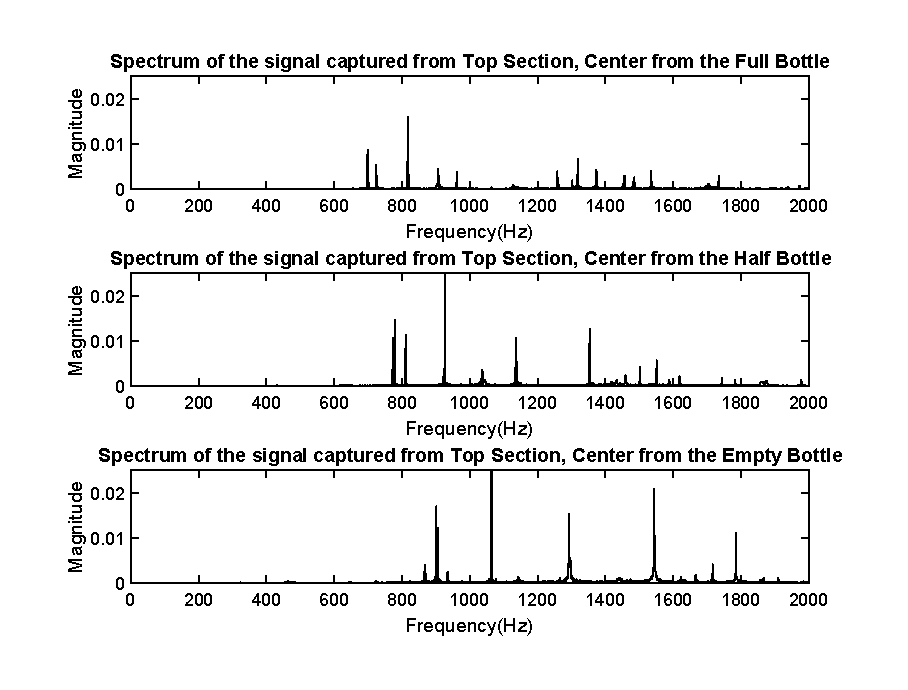
\includegraphics[width=\linewidth]{Chapters/6CHP/Figures/TopCenter.eps}
        \caption{Top Section, Center Position}{}
        \label{subfig:TopCenMic}
    \end{subfigure}
    \caption{Processed Signals in different locations in the \acrshort{lpg} bottle}{}
     \label{fig:ProcRealDataMic}
\end{figure}

After processing the data from the results obtained, observed in the figure~\ref{fig:ProcRealDataMic}, one obvious conclusion is that the signal measured at the lower section in the bottom, in figures\ref{subfig:timeLowBotMic} and~\ref{subfig:LowBotMic} doesn't result in a signal with the same amplitude in the time domain nor the same magnitude in the frequency domain, for analysis of the results this point was discarded. From the remaining points they both show some similarities, with the best results obtained in the top section in the center\ref{subfig:TopCenMic}. Comparing the lower section in the center and the top section in the bottom, the results are slightly better in the second point mentioned, although for future measurements, the point considered will depend on the results obtained when changing the sensor in use.

To reduce the amount of time used in the identification of the liquid level, it is interesting to be able to determine a frequency interval to search, the limits of the interval should be determined by the response in frequency of a full and an empty \acrshort{lpg} bottle. The results obtained from the points considered show that, isn't identify for the full bottle any frequency in the system response below the $+/-700Hz$, for the other two bottles this value increases, for the bottle half filled the value shifts to $+/-800Hz$ and for the empty bottle to $+/-900Hz$, with this in mind the lower limit for the searching interval can be set around $+/-650Hz$, to have a margin. This shift in frequency from one bottle to another can be considered as a identification method, since the first peak occurs, according to the obtained results, between the $700Hz$ to $900Hz$.

From the first peak observed in the system response, it is visible the increase in magnitude of the following peaks, until reaches a certain value where it starts to decrease again, where it starts to increase once again. Where the pattern starts to repeat, can be defined as the limit of searching. If observed, it starts to repeat around $400Hz$ after the first peak is identified, this can be used in combination to the identification of the first peak to check if after $+/-400Hz$, the identified peak has a higher magnitude than the previous, meaning that the pattern is repeating once again.

Another thing that is characteristic in the response to a stimulation of each bottle, is observed that the peak with the highest magnitude also shifts in frequency, in the interval of $+/-400Hz$ this value is approximately in the middle of this interval. For instance, for the full bottle the highest peak is around $800Hz$ and for the empty bottle is around $1100Hz$. Note that these results apply only for the results obtained at the top section and this identification method is the most inconstant, probably due the fact that the hitting is manual. Although this is not as certain as the mentioned before, these peaks also shift in frequency, which means that the searching for a peak in this interval is also valid for the liquid level identification, if combined with the other characteristics identified.

Another characteristic that must be taken in consideration, not specific to the identification, is the smaller peaks that may appear close to the ones registered, with smaller magnitude, but if what is near each one of the peaks as a sum of the surrounding, may help in the identification, this isn't mandatory to use in the identification but must be considered when developing the method to identify the liquid level.
%% Is really necessary?
To sum-up, in the development of a method to identify the liquid level should be considered the following three characteristics:
\begin{itemize}
    \item The interval on which the first peak will appear, between $650Hz$ and $950Hz$ approximately;
    \item The frequency were starts the repetition pattern, around $400Hz$ after appearing the first peak;
    \item The interval on which the peaks with the highest magnitude appear, between $800Hz$ and $1100Hz$ approximately. 
\end{itemize}

\section{Accelerometer and PiezoElectric Tests}

In chapter ~\ref{chap:hardware}, section ~\ref{sec:CaptureCoupling} several methods to mount the sensors were presented. From those, 3 different methods to mount the accelerometer in the \acrshort{lpg} and 2 for the piezoelectric. The purpose of this is to test the sensors and find the most reliable mount method, to measure the liquid level.

Beside the mounting method is important to verify how the stimulation of the bottle affects the response of the system and thus the obtained results from the sensors in use. Considering this, in the performed measurements, the stimulation was always in two different ways, manually with a hammer hitting the surface of the \acrshort{lpg}, and automatically with an impulse created with a solenoid.

The setups in the measurements, for the different stimulation methods, will be explained and the results obtained for each one of them will be analyzed in the continuation of this section.
\subsection{Stimulation and Vibration Measuring}
%Explain why only 2 stops for measurements were considered
Even though that in section ~\ref{sec:MicroTests} of this chapter, was considered four different points to perform measurements, in this case it was considered only two of those four point, mainly due the fact that for the dual magnet mount it wasn't practical to place the printed piece in the bottle. From the measuring points presented in figure ~\ref{fig:measPointMic}, was only considered the center points in both lower and top sections of the bottle.

%In both cases, manual or automatic, the software used is the same in both sensors used. 
The configurations used to sampling the signal for the different sensors were similar, since both amplifier circuits have their output centered in half of the supply voltage. So, in each one of the sampling manners used to sampling the signals, refer to the both cases. 
% Explain how the signal is capture when Manual
%\subsubsection*{Manual Stimulation}

% Explain how the signal is capture when automatic
%\subsubsection*{Automatic Stimulation}
 
\begin{description}
    \item[Manual Stimulation]{- After configuring all the peripherals necessary, a externa interruption is set to be triggered with a push-button, when pressed it enables the timer to control the sampling frequency, and starts to read the value from the analog input. The read values aren't stored right away, wait until a certain input value is reached, it is set to be under/above 128 from the mid value, this value is only passed if we knock on the bottle. From this point 1024 samples are stored and then sent via \acrshort{uart} to the computer.}
      
    \item[Automatic Stimulation]{- Similar to the manual stimulation read, the peripherals are configured and the same external interruption is set. When pushed, the interruption will activate a timer that actuates in the solenoid, simulating the impulse desire to stimulate the system. Right after stimulation the system, the timer responsible for the sampling, is activated and the conversion starts, storing 1024 samples, which are sent via \acrshort{uart} to the computer.} 

\end{description}
On the computer side, the data is received from \acrshort{uart} and stored with the use of \acrshort{matlab}. In order to analyze the data acquired with the sensors, first is used \acrshort{matlab}, which allows for a faster method to process the data and plot the results for the analysis. Before process the data in the \acrshort{fft} algorithm implemented in the microcontroller, a visual analysis must be performed to verify what are the characteristics of the processed signals, in each configuration, to later identify what is the proper method to identify the liquid level.  
%Draw fluxograms
%Explain how the data will be analyzed in the matlab
\subsection{Results}
Several measurements were performed with the different sensors, in the different locations, configurations and stimulations. The considered aspects for the measurements, although already mentioned previously, where done as follows:
\begin{enumerate}
    \item The measuring Point
    \begin{enumerate}
        \item Center, Lower Section;
        \item Center, Upper Section;
    \end{enumerate}
    \item The Stimulation Method
    \begin{enumerate}
        \item Manual, with a hammer;
        \item Automatic, with a solenoid;
    \end{enumerate}
    \item The Sensors
    \begin{enumerate}
        \item Small PiezoElectric with the sponge;
        \item PiezoElectric in a slot inside the piece;
        \item Accelerometer with the sponge;
        \item Accelerometer attached to the bottle with a magnet;
        \item Accelerometer attached to the bottle with a load strap; 
    \end{enumerate}
\end{enumerate}
From the combination of all this aspects, the results obtained are the following:
%plot the results One sensor at a time with automatic and manual side by side, the first 2 the lower section, the second 2 the top section
% LOW Manual || LOW Automatic
% UP Manual  || UP Automatic
%Accelerometer load strap
\begin{figure}[]
    \centering
    %Low
    \begin{subfigure}{0.45\textwidth}
        \centering
        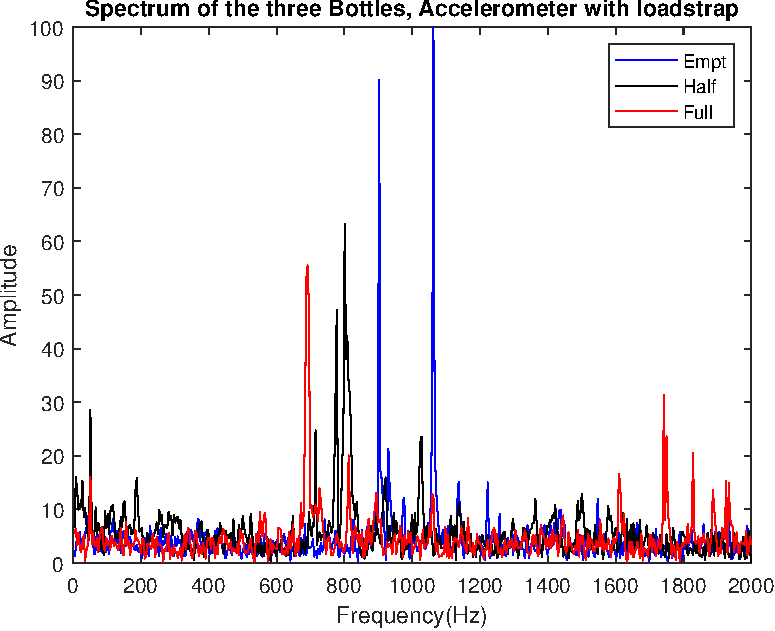
\includegraphics[width=\linewidth]{Chapters/6CHP/Figures/ResultsSensors/AcCiMaBot.pdf}
        \caption{Manual Stimulation at the center of the lower section}{}
        \label{subfig:ResAcCiMaBot}
    \end{subfigure}
    \begin{subfigure}{0.45\textwidth}
        \centering
        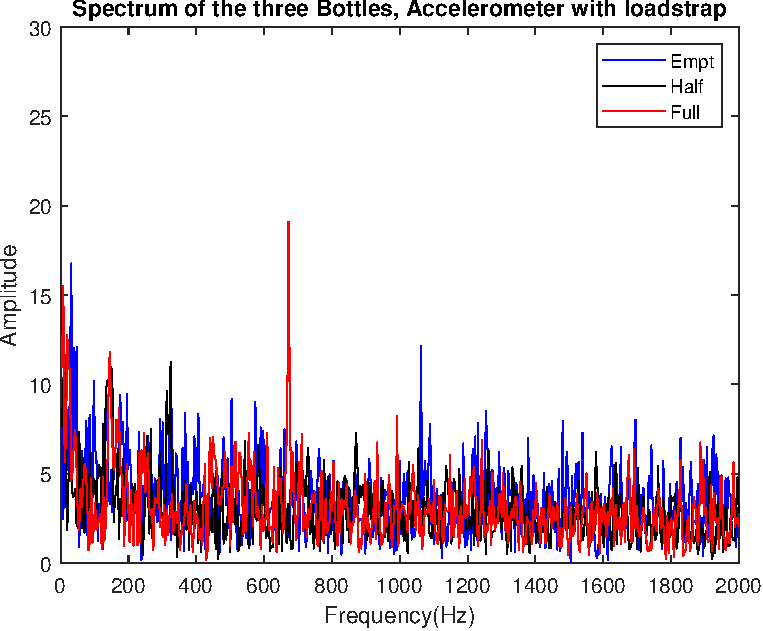
\includegraphics[width=\linewidth]{Chapters/6CHP/Figures/ResultsSensors/AcCiAuBot.pdf}
        \caption{Automatic Stimulation at the center of the lower section}{}
        \label{subfig:ResAcCiAuBot}
    \end{subfigure}
    %Up
    \begin{subfigure}{0.45\textwidth}
        \centering
        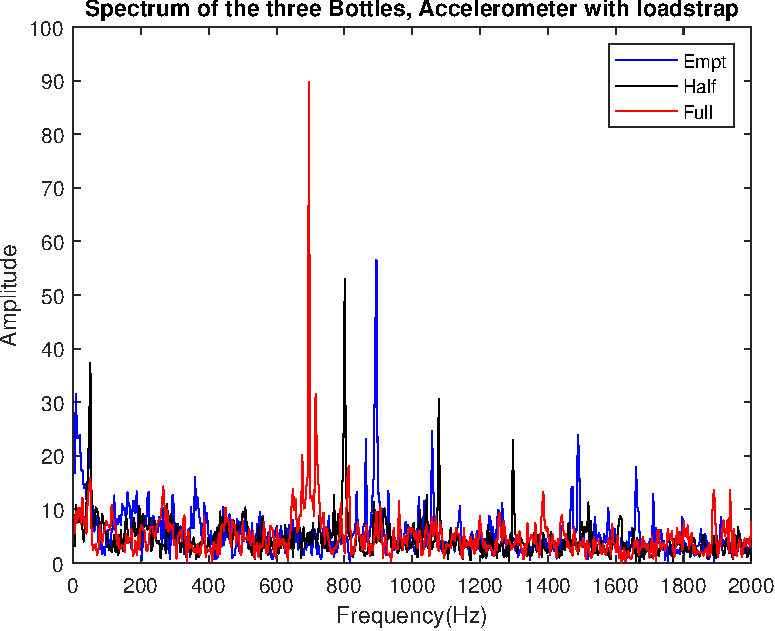
\includegraphics[width=\linewidth]{Chapters/6CHP/Figures/ResultsSensors/AcCiMaTop.pdf}
        \caption{Manual Stimulation at the center of the upper section}{}
        \label{subfig:ResAcCiMaTop}
    \end{subfigure}
    \begin{subfigure}{0.45\textwidth}
        \centering
        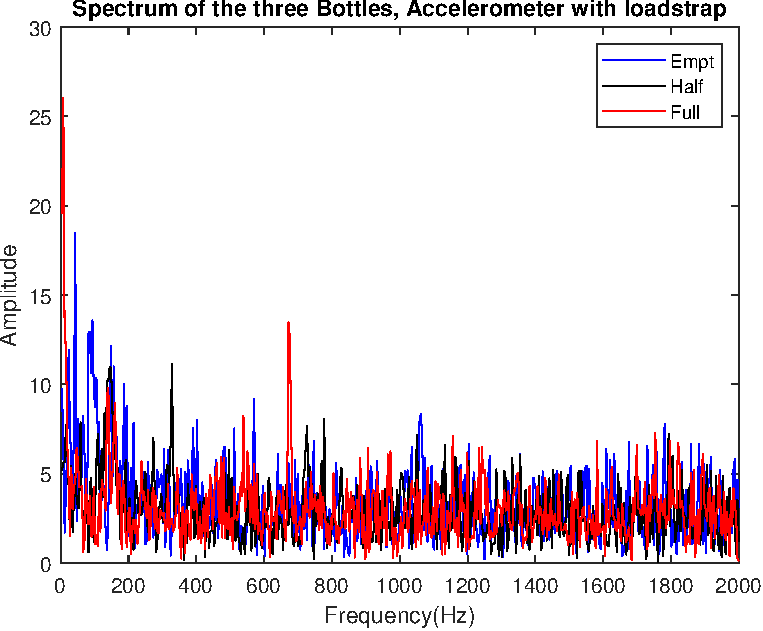
\includegraphics[width=\linewidth]{Chapters/6CHP/Figures/ResultsSensors/AcCiAuTop.pdf}
        \caption{Automatic Stimulation at the center of the upper section}{}
        \label{subfig:ResAcCiAuTop}
    \end{subfigure}
    \caption{Accelerometer attached to the bottle with a load strap}{}
    \label{fig:AccLoadStrap}
\end{figure}
%Accelerometer magnet
\begin{figure}[]
    \centering
    %Low
    \begin{subfigure}{0.45\textwidth}
        \centering
        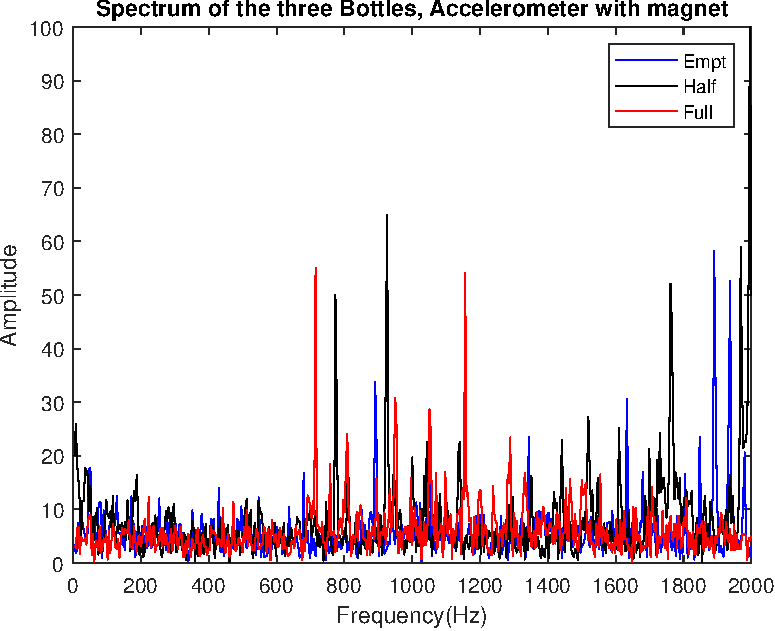
\includegraphics[width=\linewidth]{Chapters/6CHP/Figures/ResultsSensors/AcImMaBot.pdf}
        \caption{Manual Stimulation at the center of the lower section}{}
        \label{subfig:ResAcImMaBot}
    \end{subfigure}
    \begin{subfigure}{0.45\textwidth}
        \centering
        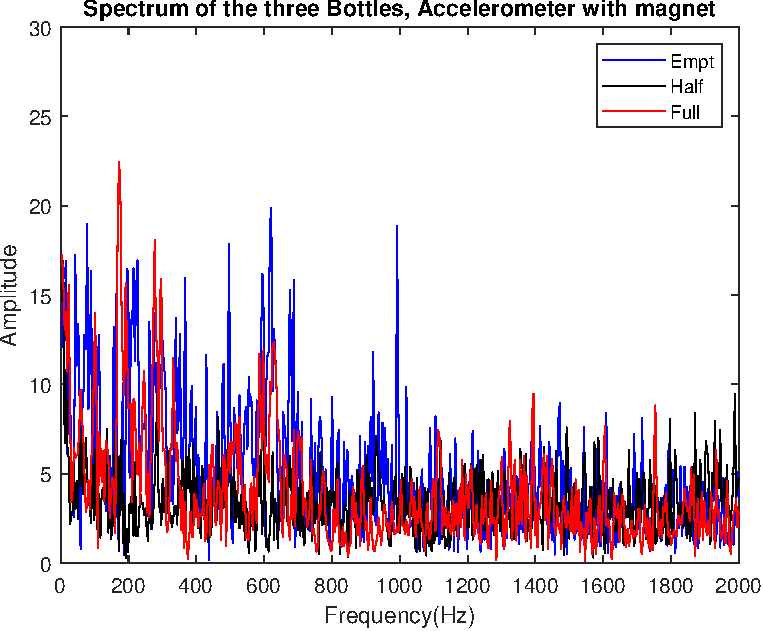
\includegraphics[width=\linewidth]{Chapters/6CHP/Figures/ResultsSensors/AcImAuBot.pdf}
        \caption{Automatic Stimulation at the center of the lower section}{}
        \label{subfig:ResAcImAuBot}
    \end{subfigure}
    %Up
    \begin{subfigure}{0.45\textwidth}
        \centering
        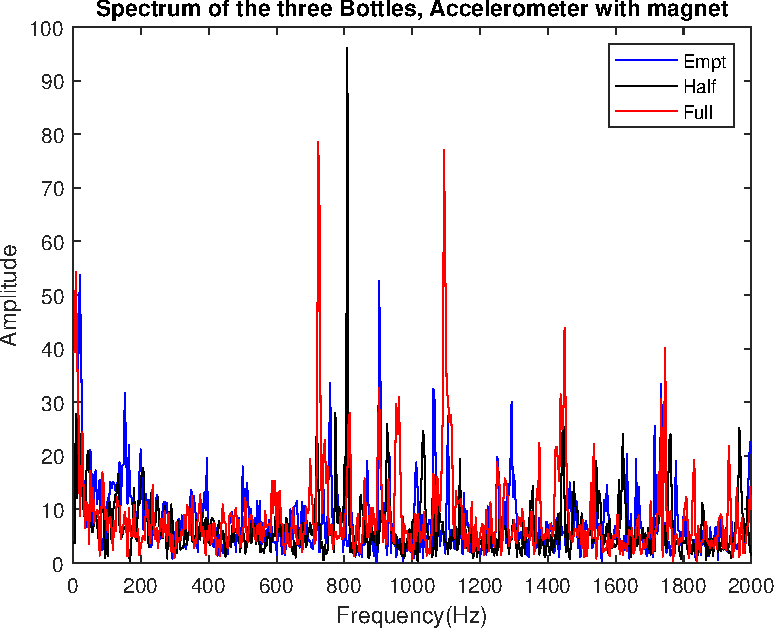
\includegraphics[width=\linewidth]{Chapters/6CHP/Figures/ResultsSensors/AcImMaTop.pdf}
        \caption{Manual Stimulation at the center of the upper section}{}
        \label{subfig:ResAcImMaTop}
    \end{subfigure}
    \begin{subfigure}{0.45\textwidth}
        \centering
        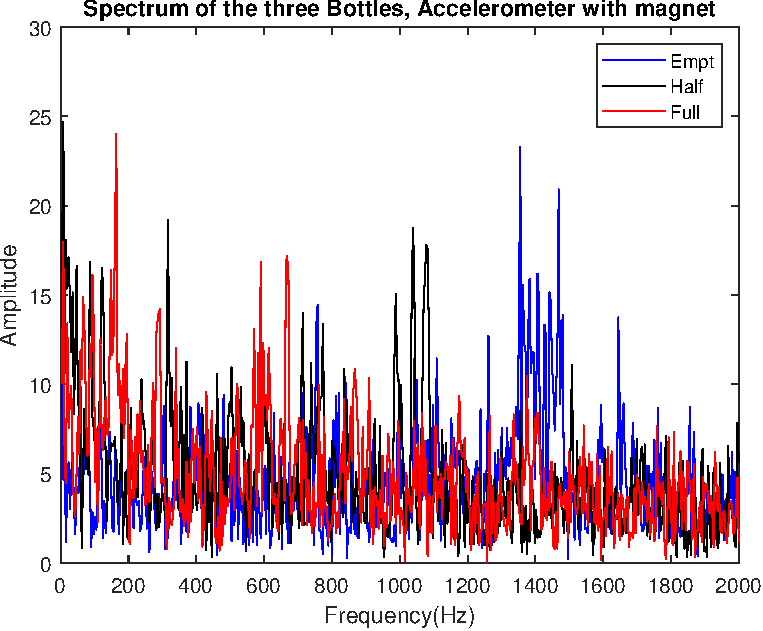
\includegraphics[width=\linewidth]{Chapters/6CHP/Figures/ResultsSensors/AcImAuTop.pdf}
        \caption{Automatic Stimulation at the center of the upper section}{}
        \label{subfig:ResAcImAuTop}
    \end{subfigure}
    \caption{Accelerometer attached to the bottle with a magnet}{}
    \label{fig:AccMagnet}
\end{figure}
%Accelerometer sponge
\begin{figure}[]
    \centering
    %Low
    \begin{subfigure}{0.45\textwidth}
        \centering
        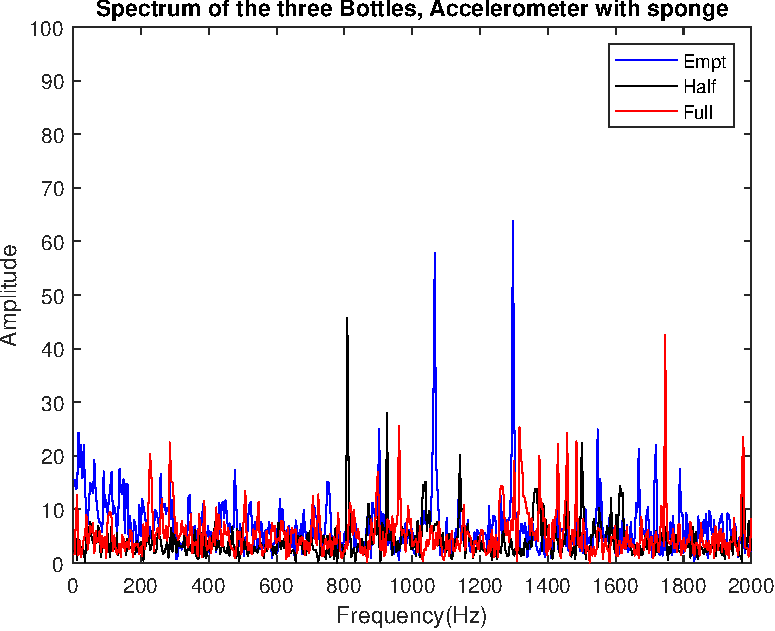
\includegraphics[width=\linewidth]{Chapters/6CHP/Figures/ResultsSensors/AcEsMaBot.pdf}
        \caption{Manual Stimulation at the center of the lower section}{}
        \label{subfig:ResAcEsMaBot}
    \end{subfigure}
    \begin{subfigure}{0.45\textwidth}
        \centering
        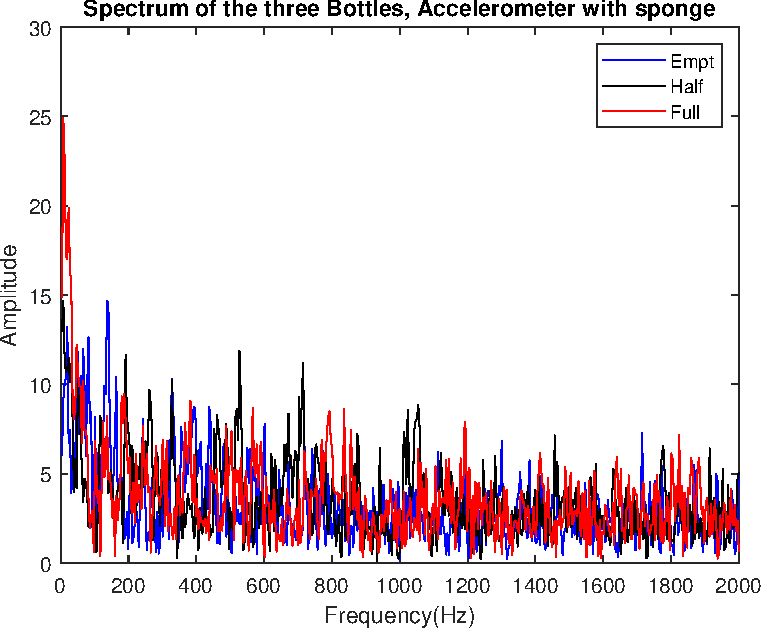
\includegraphics[width=\linewidth]{Chapters/6CHP/Figures/ResultsSensors/AcEsAuBot.pdf}
        \caption{Automatic Stimulation at the center of the lower section}{}
        \label{subfig:ResAcEsAuBot}
    \end{subfigure}
    %Up
    \begin{subfigure}{0.45\textwidth}
        \centering
        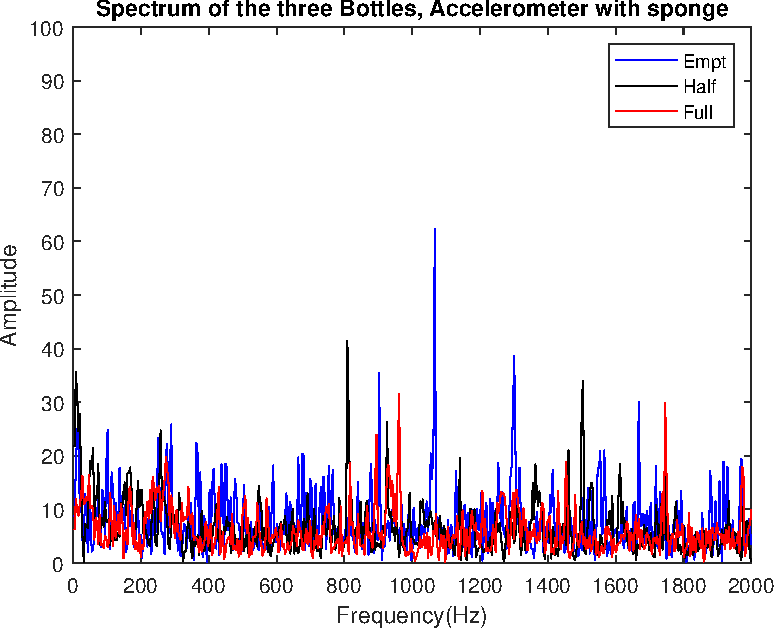
\includegraphics[width=\linewidth]{Chapters/6CHP/Figures/ResultsSensors/AcEsMaTop.pdf}
        \caption{Manual Stimulation at the center of the upper section}{}
        \label{subfig:ResAcEsMaTop}
    \end{subfigure}
    \begin{subfigure}{0.45\textwidth}
        \centering
        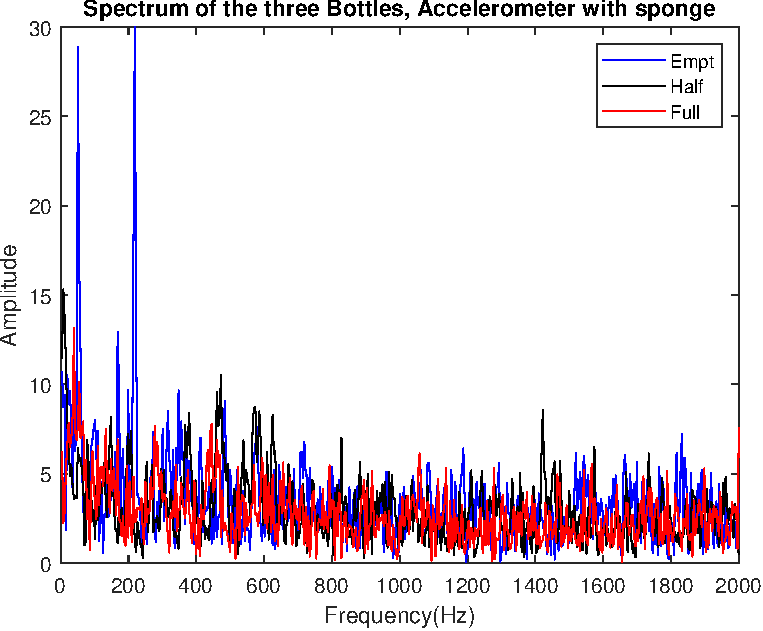
\includegraphics[width=\linewidth]{Chapters/6CHP/Figures/ResultsSensors/AcEsAuTop.pdf}
        \caption{Accelerometer attached to the bottle with a load strap}{}
        \label{subfig:ResAcEsAuTop}
    \end{subfigure}
    \caption{Accelerometer attached to the bottle with a dual mount magnet and a sponge}{}
    \label{fig:AccSponge}
\end{figure}
%Piezo Big
\begin{figure}[]
    \centering
    %Low
    \begin{subfigure}{0.45\textwidth}
        \centering
        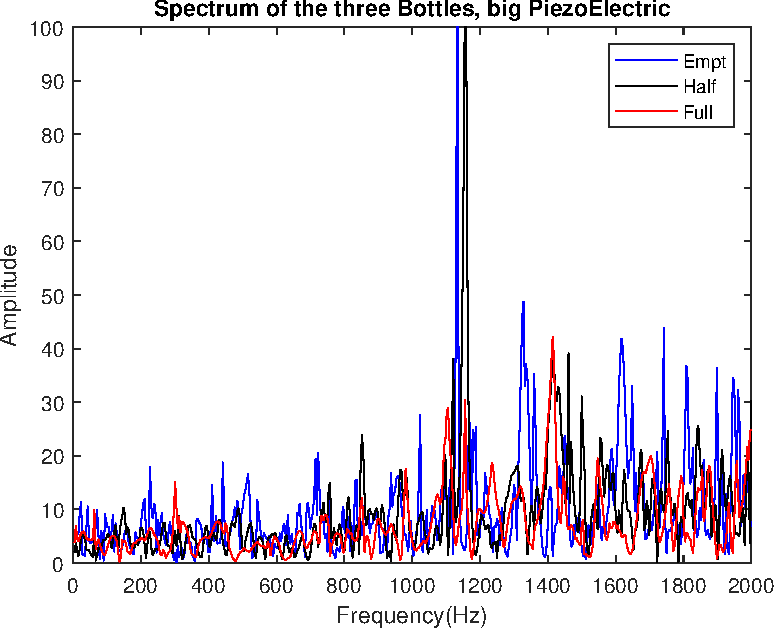
\includegraphics[width=\linewidth]{Chapters/6CHP/Figures/ResultsSensors/PiezBMaBot.pdf}
        \caption{Manual Stimulation at the center of the lower section}{}
        \label{subfig:ResPiezBMaBot}
    \end{subfigure}
    \begin{subfigure}{0.45\textwidth}
        \centering
        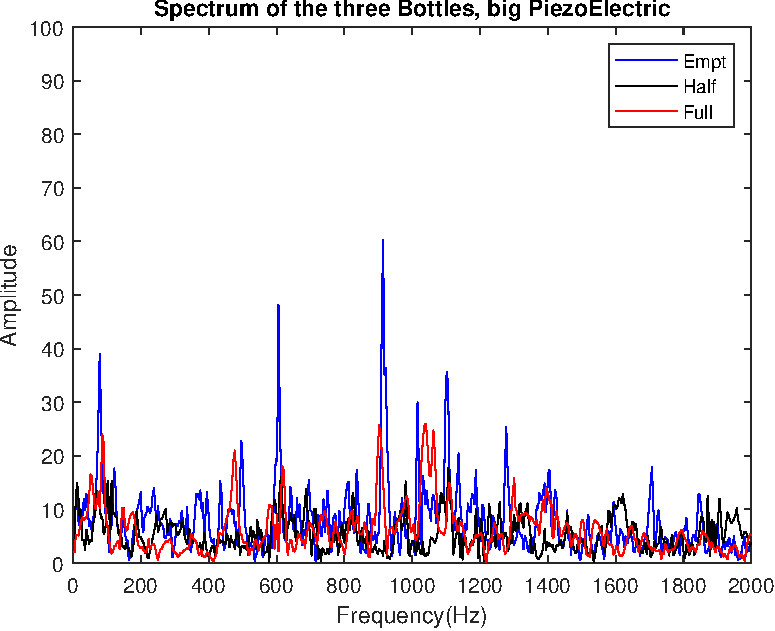
\includegraphics[width=\linewidth]{Chapters/6CHP/Figures/ResultsSensors/PiezBAuBot.pdf}
        \caption{Automatic Stimulation at the center of the lower section}{}
        \label{subfig:ResPiezBAuBot}
    \end{subfigure}
    %Up
    \begin{subfigure}{0.45\textwidth}
        \centering
        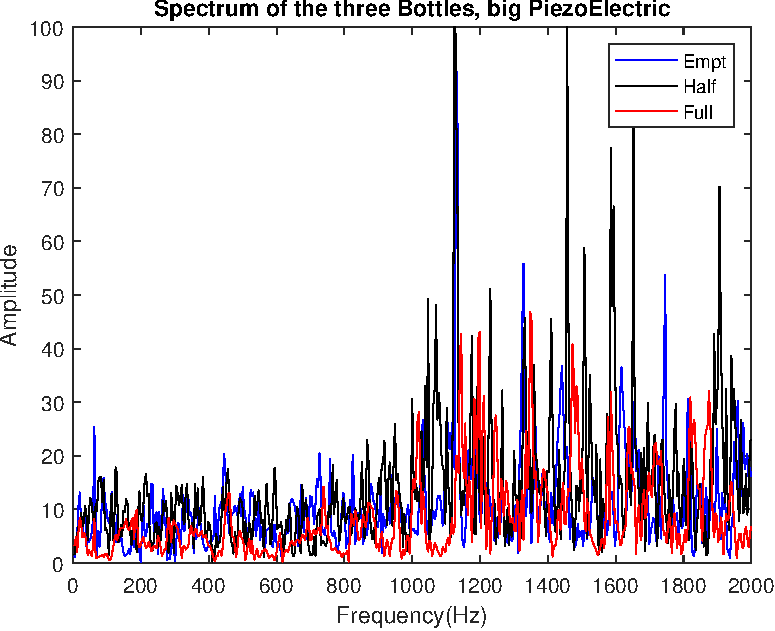
\includegraphics[width=\linewidth]{Chapters/6CHP/Figures/ResultsSensors/PiezBMaTop.pdf}
        \caption{Manual Stimulation at the center of the upper section}{}
        \label{subfig:ResPiezBMaTop}
    \end{subfigure}
    \begin{subfigure}{0.45\textwidth}
        \centering
        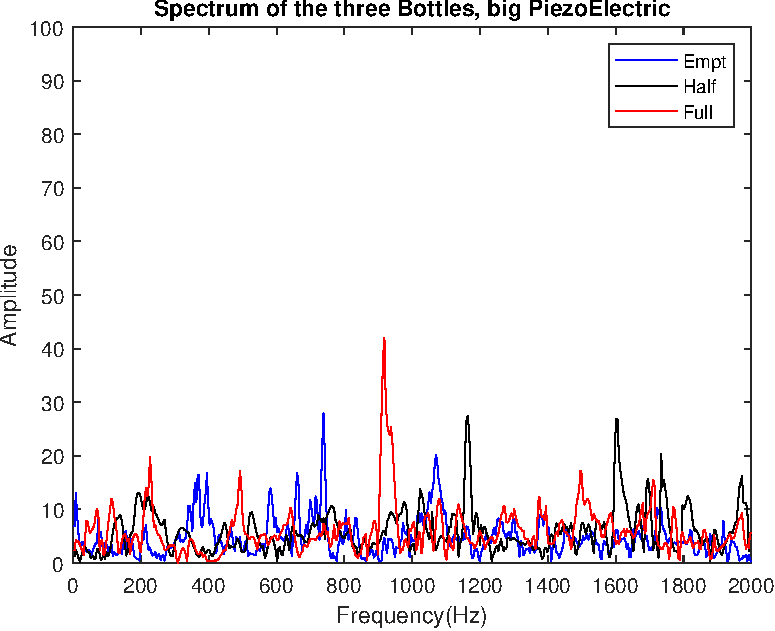
\includegraphics[width=\linewidth]{Chapters/6CHP/Figures/ResultsSensors/PiezBAuTop.pdf}
        \caption{Accelerometer attached to the bottle with a load strap}{}
        \label{subfig:ResPiezBAuTop}
    \end{subfigure}
    \caption{Big PiezoElectric inserted in a slot of a dual mount magnet piece}{}
    \label{fig:PiezB}
\end{figure}
%piezo small
\begin{figure}[]
    \centering
    %Low
    \begin{subfigure}{0.45\textwidth}
        \centering
        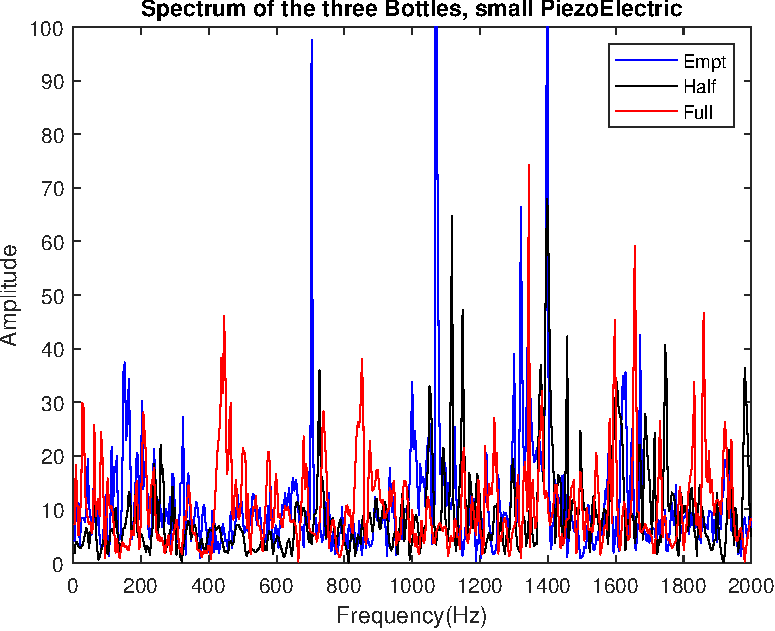
\includegraphics[width=\linewidth]{Chapters/6CHP/Figures/ResultsSensors/PiezzMaBot.pdf}
        \caption{Manual Stimulation at the center of the lower section}{}
        \label{subfig:ResPiezzMaBot}
    \end{subfigure}
    \begin{subfigure}{0.45\textwidth}
        \centering
        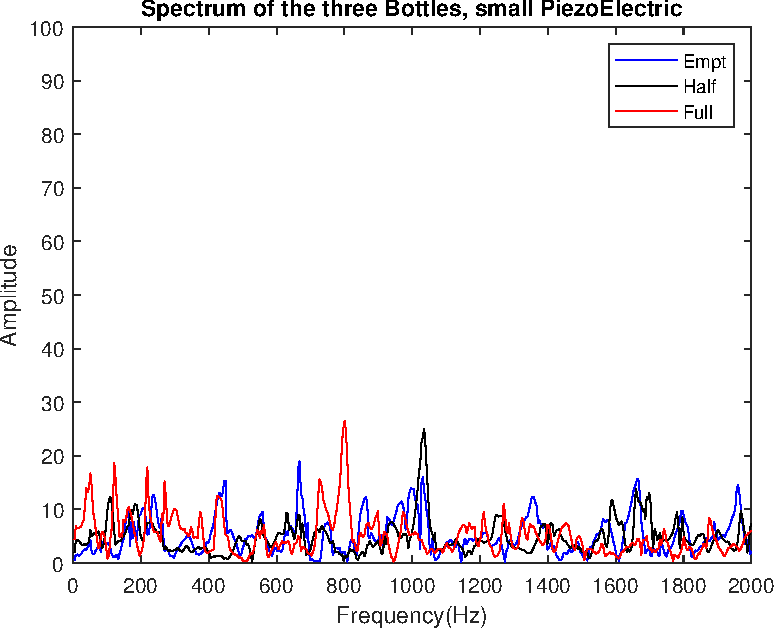
\includegraphics[width=\linewidth]{Chapters/6CHP/Figures/ResultsSensors/PiezzAuBot.pdf}
        \caption{Automatic Stimulation at the center of the lower section}{}
        \label{subfig:ResPiezzAuBot}
    \end{subfigure}
    % Up
    \begin{subfigure}{0.45\textwidth}
        \centering
        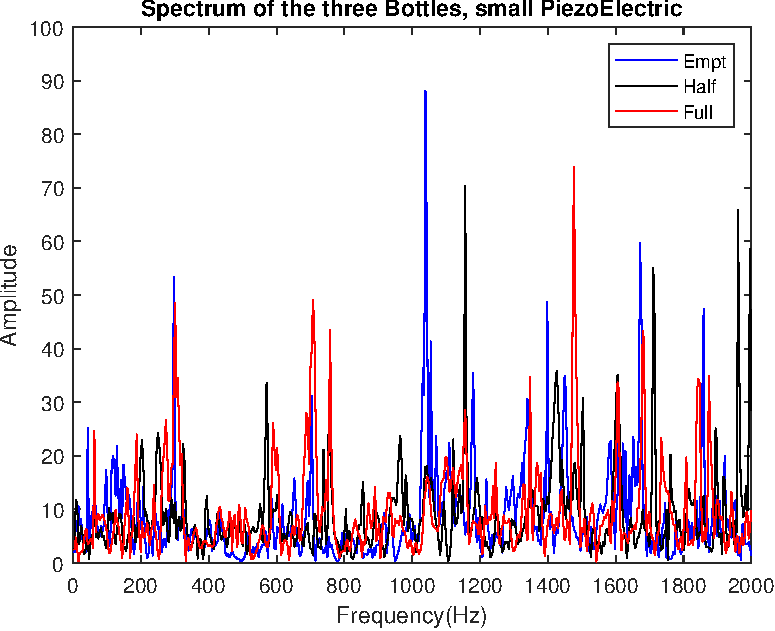
\includegraphics[width=\linewidth]{Chapters/6CHP/Figures/ResultsSensors/PiezzMaTop.pdf}
        \caption{Manual Stimulation at the center of the upper section}{}
        \label{subfig:ResPiezzMaTop}
    \end{subfigure}
    \begin{subfigure}{0.45\textwidth}
        \centering
        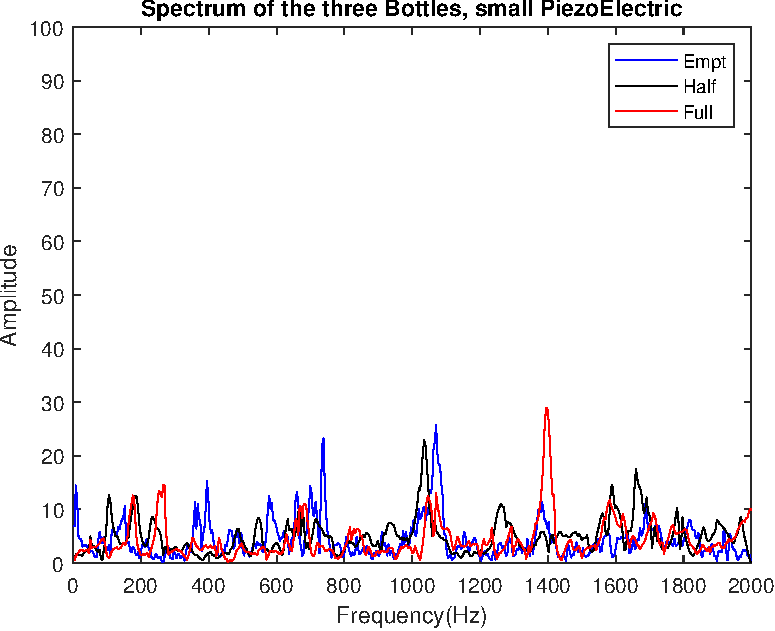
\includegraphics[width=\linewidth]{Chapters/6CHP/Figures/ResultsSensors/PiezzAuTop.pdf}
        \caption{Accelerometer attached to the bottle with a load strap}{}
        \label{subfig:ResPiezzAuTop}
    \end{subfigure}
    \caption{Small PiezoElectric attached with a dual magnet mount and a sponge}{}
    \label{fig:Piezz}
\end{figure}
% analyze the results
\todo[inline,color=red!40]{*Add link to the remaining results if necessary and addapt the first paragraph that follows to lead to the results latter!}
Note that the presented results in the images above, are only referring to one sample of each bottle in each setup. In overall, at least 10 measurements in each point and setups were performed, most of the measurements repeated more than once with small adjustments, at the hardware or software. The presented ones refer to the last series of measurements. %Add reference to the folder were are the remaining results??

From all the results presented for the different setups, one thing is clear, the use of the solenoid for the automatic stimulation was a complete failure, none of the presented graphics on that setup provided relevant information about the liquid level, this lead to the conclusion that the stimulation with the solenoid isn't enough to the accelerometer or the piezoelectric sensor determine the variation in vibration for the different bottles, as is going to be proved when analyzing the manual stimulation. 

This may be due the fact that the impact caused with the solenoid isn't enough to produce a visible vibration of the systems that surpasses the natural oscillation of the output of the sensors, that after being amplified results in noise. Although the noise is a problem, this could be bypassed by averaging, different spectrums of different measurements in the same conditions, this results in a decrease of the noise but without the expected results, the spectrum obtained still returned random values, without clear information.

From the results obtained with the manual stimulation, the conclusions are the same as above, with two exceptions. Those were by using the accelerometer attached with a load strap and one magnet. From these two, the most clear results are in the accelerometer attached with a load strap, but is also visible a pattern between the three bottles, with the first highest peaks occurring between $+/- 700Hz$ to the $+/-900Hz$, from the full to the empty bottle. The same results are also visible with the magnet, but with the introduction of more peaks in between with smaller amplitudes, this is reduced when averaging the spectrum.

Another thing that is important to mention is that even though several measurements with the piezoelectric were performed, none of them presented relevant information, not even when averaging the spectrum. In the different tests it was never clear what was the reason why the piezoelectric haven't any valid results. 
%conclusions
Considering the presented setups, is only going to be used in future analysis the two setups that have shown some results, that are the accelerometer with one magnet and the load strap. One final conclusion to take from all performed measurements, is how much the impact affects the response of the system and thus the acquired signal with the sensor, as well as the mounting of the sensor plays an important role in the captured vibration.
\section{Identification algorithm Tests}
% what signals where considered
At this stage is important to move from the tests and analysis with \acrshort{matlab} and verify if the algorithm implemented in the microcontroller returns similar results, for this were considered the signals obtained with the microphone, the accelerometer with the load strap and the accelerometer with the magnet. The signals captured with the microphone were used because their spectrum was less noisy than the spectrum from the other sensors, if the identification didn't work with these signals, it wouldn't for sure to work with the remaining. Also, they were used as a way to define the limits of search in the identification algorithm, i.e. to define the interval in frequency to the identification of the liquid level.  
% How the tests were performed
\subsection{Identification Steps??}
The first step was to obtain the spectrum of signals from the three different bottles, to define the interval in frequency in order to reduce the amount of time in the search having more accuracy. In this case, the original signal was cropped and sent to the microcontroller for processing, returning then to the computer for analysis.

After this, an interval was determined and the identification algorithm was developed to find the liquid level. What it does is, a threshold value is determined between a relation of the average amplitude of the spectrum and the highest peak, this allows for the threshold value to vary according to the amplitude of the signal. This threshold value is what determines if it is a important peak, or is just noise related. 

Considering this threshold value and the limits defined, three main functions were created. The first one identifies the first peak, starts to look in the lower limit and goes until the upper limit, when find the first value above the threshold value, the function stops and returns the value.

The second function considers a different limit, the lower is the same as in the first situation, the upper is set according to the cutoff frequency of the accelerometer, when testing with their values, otherwise is set until half of the sampling frequency. This function finds the highest peak in the spectrum, search for the entire spectrum considered and when ends returns the value of the highest one.

The third function was developed, to try to bypass one thing that was noticed in the second, most of the times the highest peaks match with the first peak, which is due the inconsistency of the knock. When this occurs, near the frequency where it usually occurs, the spectrum has smaller peaks around it instead of a highest one, this was the way to try to find the consistency, by averaging around each peak and determine which one of them has the highest energy. The purpose of this third function is exactly this and return the value of where this happens.

Considering the functions for the identification of the liquid level, the signals obtained with the microphone, and the two configurations with the accelerometer, were sent to the microcontroller for identification and processing and the results of the identification returned to the computer. On the computer side the results were plotted in order to find how well the identification functions worked. 

One thing important to mentioned is, the only reason that the definition of the threshold value is this way is, since the manual hitting produces different responses, the algorithm needs to adapt to that variation, if the process was automatic this probably wouldn't be necessary, was expected to have consistent between all the signal captured to the same point.   
\subsection{Results}
Before getting into the results obtained from the function created for the identification, the spectrum obtained from the processing with the microcontroller was analyzed, both in the microphone and the accelerometer, in the figure ~\ref{fig:specuC} is presented the results.
\begin{figure}[]
    \centering
    \begin{subfigure}{0.45\textwidth}
        \centering
        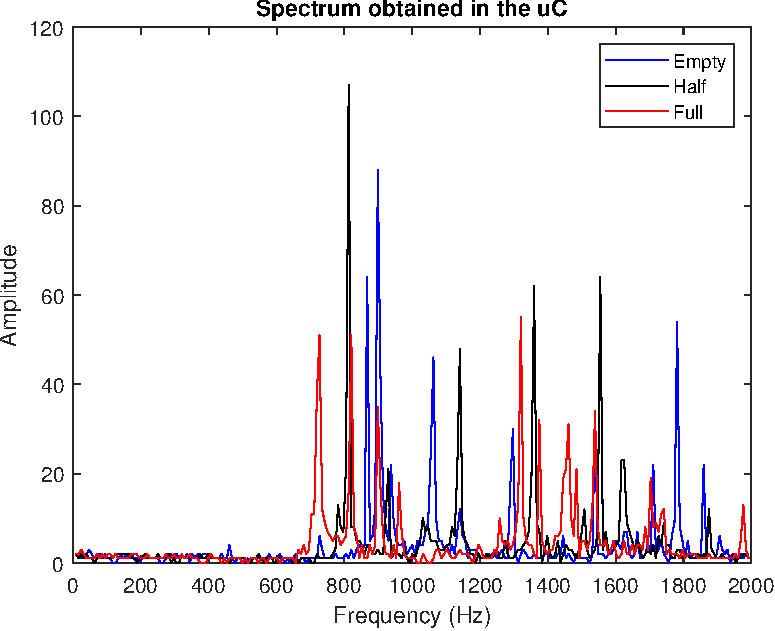
\includegraphics[width=\linewidth]{Chapters/6CHP/Figures/ResultsuCGraphs/specMICuC.pdf}
        \caption{Spectrum of the samples obtained with the microphone, for the 3 bottles}{}
        \label{subfig:specMICuc}
    \end{subfigure}
    \begin{subfigure}{0.45\textwidth}
        \centering
        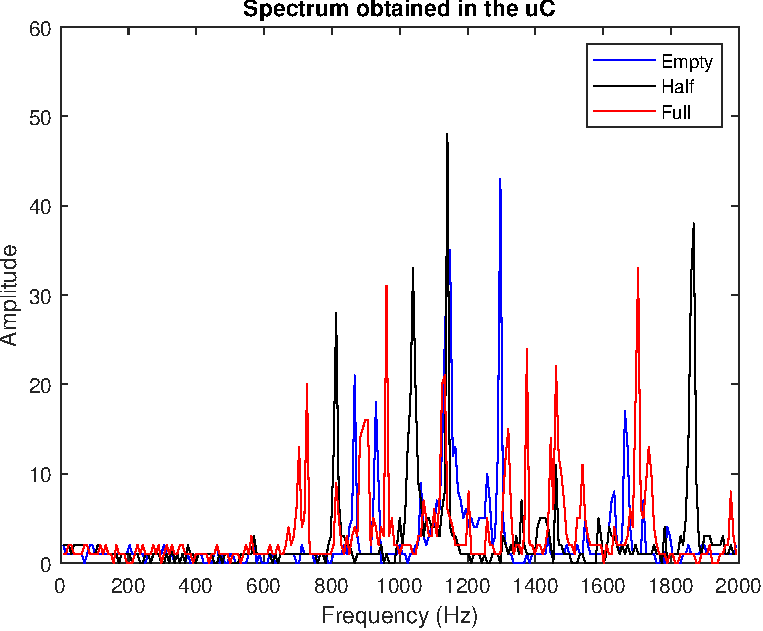
\includegraphics[width=\linewidth]{Chapters/6CHP/Figures/ResultsuCGraphs/uCGraphsSen.pdf}
        \caption{Spectrum of the samples obtained with the accelerometer with the load strap, for the 3 bottles}{}
        \label{subfig:specAccuC}
    \end{subfigure}
    \caption{Spectrum obtained by processing the signals in the microcontroller}{}
    \label{fig:specuC}
\end{figure}

From the spectrum obtained for both cases it is visible that there are not any relevant peaks below the 600Hz, in order to reduce the amount of time searching for the characteristics of the captured signals, this frequency is the reference to start. Another thing that is visible here is that it is possible to observe a shift in frequency for the first peak of the measured signal for each bottle, this can give us with certainty on method to determine the difference between the three bottles, if the other methods aren't precise.

In the following graphics is going to be presented the results obtained for the identification algorithms, for the cases mentioned previously. Is important to mention, that the results of the functions developed aren't the frequency of each peak, but the id in the vector of each peak, in the future is irrelevant to determine the liquid level if is an ID or a frequency.
%%MIC
\begin{figure}[]
    \centering
    \begin{subfigure}{0.45\textwidth}
        \centering
        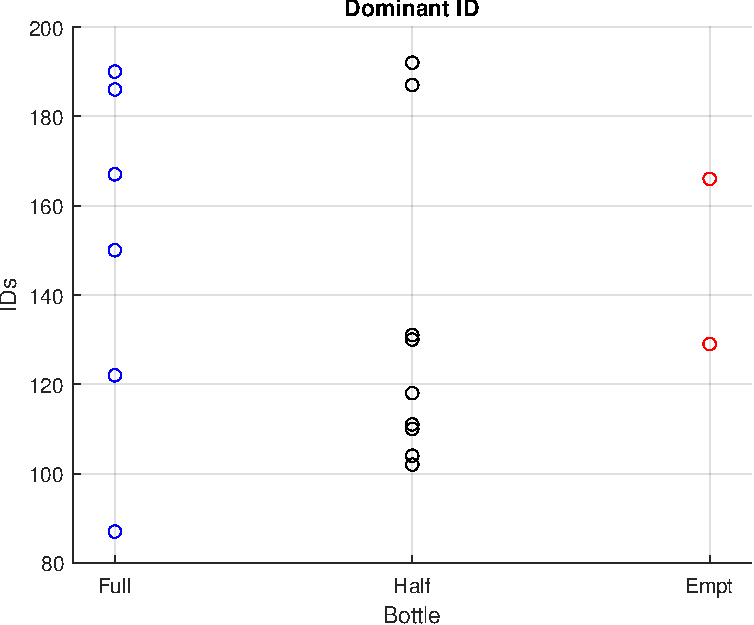
\includegraphics[width=\linewidth]{Chapters/6CHP/Figures/ResultsuCGraphs/MIC/BotMiddomID.pdf}
        \caption{Results for the search of the identify, of the dominant peak}{}
        \label{subfig:domIDMIC}
    \end{subfigure}
    \begin{subfigure}{0.45\textwidth}
        \centering
        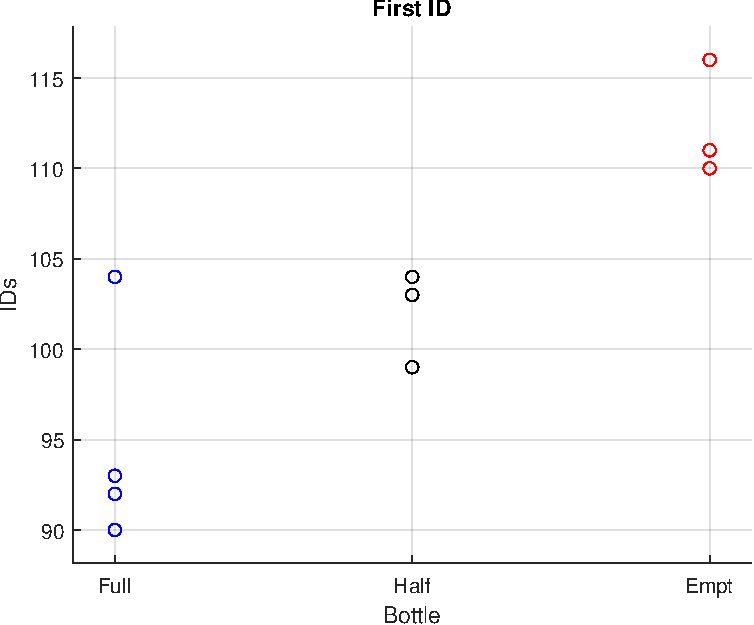
\includegraphics[width=\linewidth]{Chapters/6CHP/Figures/ResultsuCGraphs/MIC/BotMidfID.pdf}
        \caption{Results of the search of the ID, of the first peak}{}
        \label{subfig:fIDMIC}
    \end{subfigure}
    \begin{subfigure}{0.45\textwidth}
        \centering
        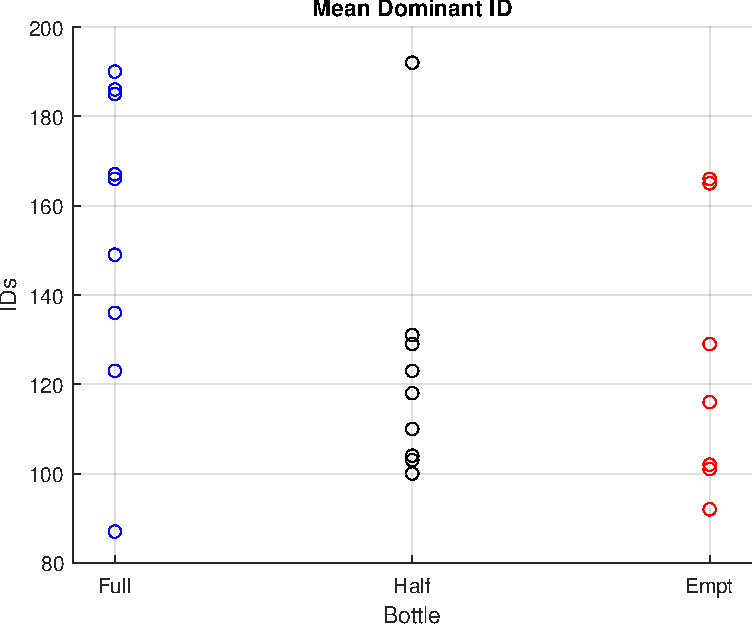
\includegraphics[width=\linewidth]{Chapters/6CHP/Figures/ResultsuCGraphs/MIC/BotMidmID.pdf}
        \caption{Results of the search of the ID, of the mean dominant peak}{}
        \label{subfig:mIDMIC}
    \end{subfigure}
    \caption{Results from the analysis of the signals obtained with the microphone, at the center of the lower section}{}
    \label{fig:MICResAlg}
\end{figure}
%%ACC with Load strap
\begin{figure}[]
    \centering
    \begin{subfigure}{0.45\textwidth}
        \centering
        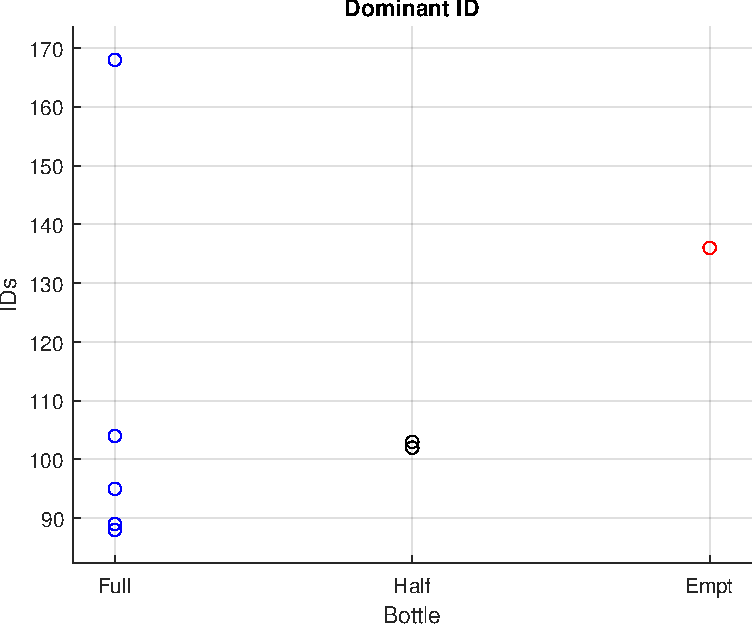
\includegraphics[width=\linewidth]{Chapters/6CHP/Figures/ResultsuCGraphs/Sen/BotMidAcCiMa18_05domID.pdf}
        \caption{Results for the search of the identify, of the dominant peak}{}
        \label{subfig:domIDACCL}
    \end{subfigure}
    \begin{subfigure}{0.45\textwidth}
        \centering
        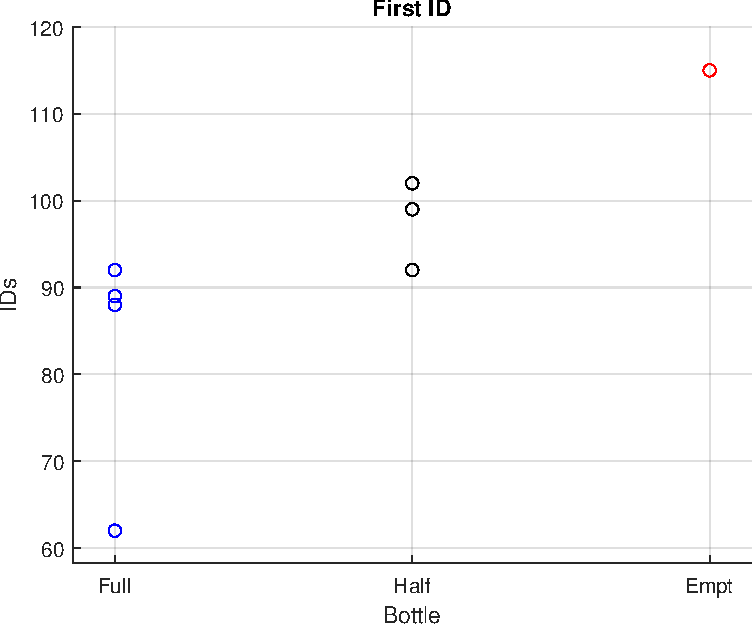
\includegraphics[width=\linewidth]{Chapters/6CHP/Figures/ResultsuCGraphs/Sen/BotMidAcCiMa18_05fID.pdf}
        \caption{Results of the search of the ID, of the first peak}{}
        \label{subfig:fIDACCL}
    \end{subfigure}
    \begin{subfigure}{0.45\textwidth}
        \centering
        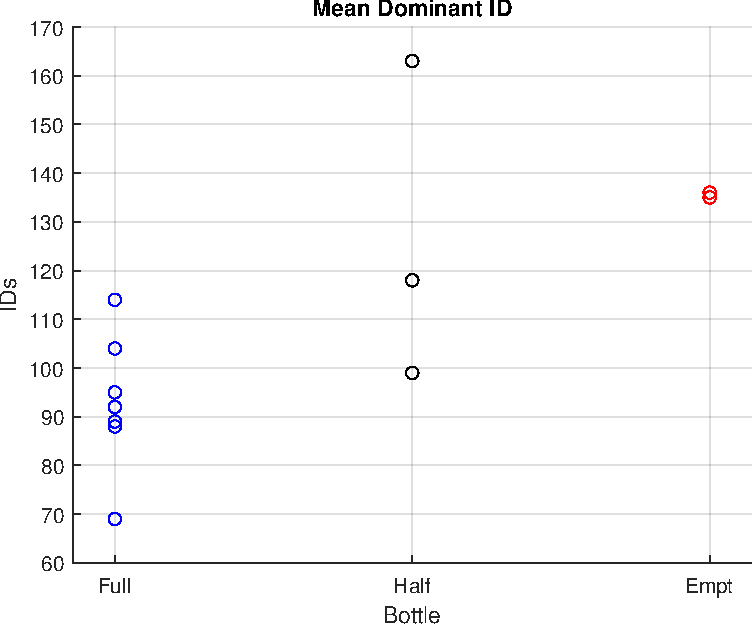
\includegraphics[width=\linewidth]{Chapters/6CHP/Figures/ResultsuCGraphs/Sen/BotMidAcCiMa18_05mID.pdf}
        \caption{Results of the search of the ID, of the mean dominant peak}{}
        \label{subfig:mIDACCL}
    \end{subfigure}
    \caption{Results from the analysis of the signals obtained with the Accelerometer with the load strap, at the center of the lower section}{}
    \label{fig:ACCLResAlg}
\end{figure}
%%ACC with magnet
\begin{figure}[]
    \centering
    \begin{subfigure}{0.45\textwidth}
        \centering
        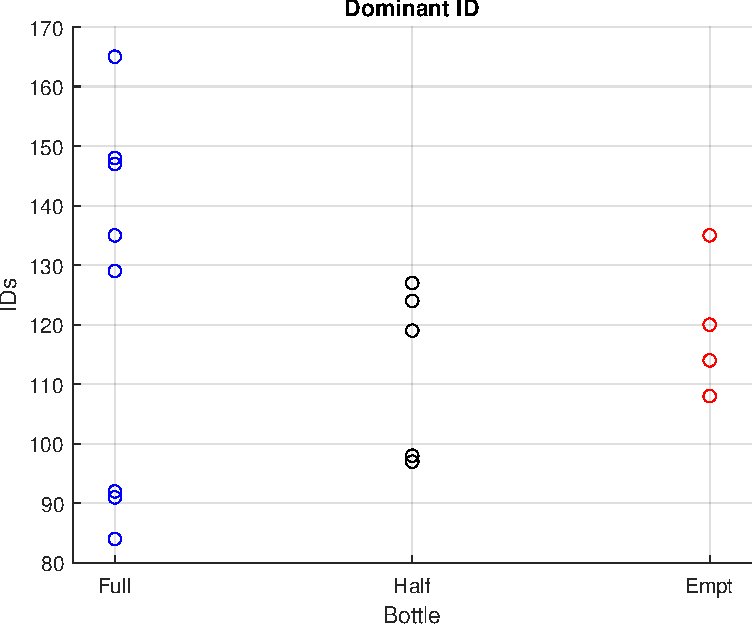
\includegraphics[width=\linewidth]{Chapters/6CHP/Figures/ResultsuCGraphs/Sen/BotMidAcImMa18_05domID.pdf}
        \caption{Results for the search of the identify, of the dominant peak}{}
        \label{subfig:domIDACCI}
    \end{subfigure}
    \begin{subfigure}{0.45\textwidth}
        \centering
        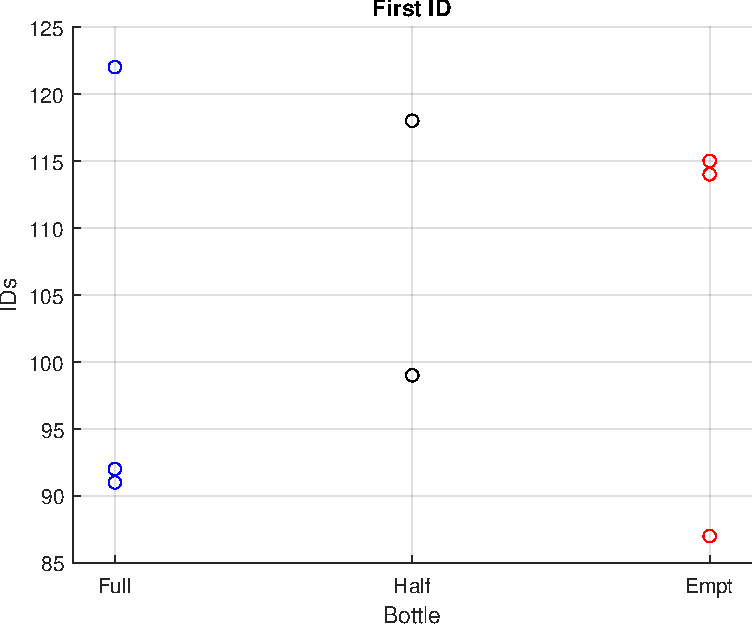
\includegraphics[width=\linewidth]{Chapters/6CHP/Figures/ResultsuCGraphs/Sen/BotMidAcImMa18_05fID.pdf}
        \caption{Results of the search of the ID, of the first peak}{}
        \label{subfig:fIDACCI}
    \end{subfigure}
    \begin{subfigure}{0.45\textwidth}
        \centering
        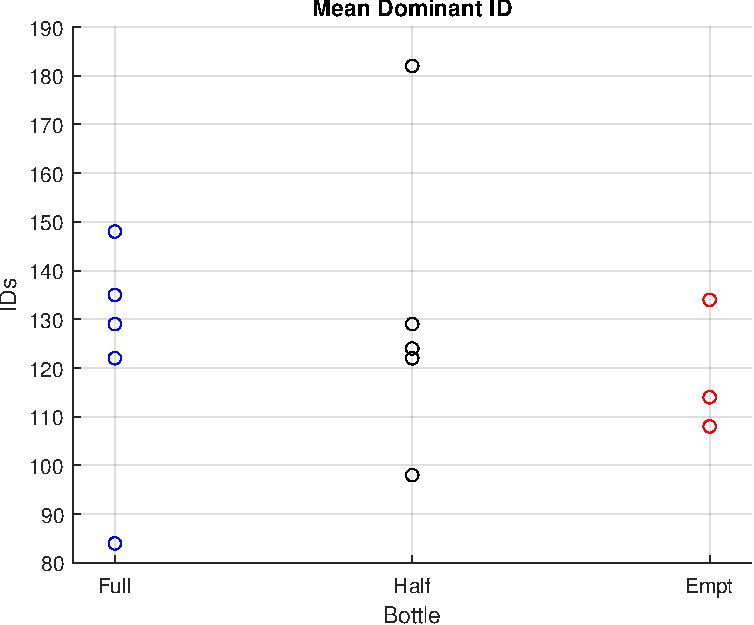
\includegraphics[width=\linewidth]{Chapters/6CHP/Figures/ResultsuCGraphs/Sen/BotMidAcImMa18_05mID.pdf}
        \caption{Results of the search of the ID, of the mean dominant peak}{}
        \label{subfig:mIDACCI}
    \end{subfigure}
    \caption{Results from the analysis of the signals obtained with the Accelerometer with the magnet, at the center of the lower section}{}
    \label{fig:ACCIResAlg}
\end{figure}
%\todo[inline,color=red!40]{Add the graphics at resulted from the top as attachement}
Note that the presented results were measured at the lower section at the center, the reason is that the results at the upper section were less precise when compared with the results presented. This also leads to the conclusion that the optimal point for the measurements should be at the lower section. 

From the results obtained, one thing is visible in all the tested setups, the most precise results were obtained in the search of the first peak, although there are some signals that are an exception, it is possible to conclude that considering the circumstances, this could be implemented with the search of the first ID. One possible reason for the exception, may be due the value of the threshold value, be variant between samples, and the stimulation isn't constant, it is possible to stimulate the system in a constant manner and strong enough to produce results similar to this, this problem will probably be bypassed. 

Is quite satisfactory to observe that there is a pattern between the three bottles that allow us to identify each one of them. If a consistency is found, the other two functions may also result in more stable results, and the three function combined can lead to more precise results.
% Add a graphics with the spectrum of the signals from the microphone obtained in the microcontroller  
%% add the rest tomorrow
From all the tests performed, in most of the cases the results obtained were satisfactory, although there are some considerations to do about them. This consideration will be explored in detail in this chapter referring to the future work~\ref{sec:FutureWork}.


\clearpage
%\printbibliography[heading=subbibliography]
%\addcontentsline{toc}{section}{References}